\documentclass[]{tufte-book}

% ams
\usepackage{amssymb,amsmath}

\usepackage{ifxetex,ifluatex}
\usepackage{fixltx2e} % provides \textsubscript
\ifnum 0\ifxetex 1\fi\ifluatex 1\fi=0 % if pdftex
  \usepackage[T1]{fontenc}
  \usepackage[utf8]{inputenc}
\else % if luatex or xelatex
  \makeatletter
  \@ifpackageloaded{fontspec}{}{\usepackage{fontspec}}
  \makeatother
  \defaultfontfeatures{Ligatures=TeX,Scale=MatchLowercase}
  \makeatletter
  \@ifpackageloaded{soul}{
     \renewcommand\allcapsspacing[1]{{\addfontfeature{LetterSpace=15}#1}}
     \renewcommand\smallcapsspacing[1]{{\addfontfeature{LetterSpace=10}#1}}
   }{}
  \makeatother

\fi

% graphix
\usepackage{graphicx}
\setkeys{Gin}{width=\linewidth,totalheight=\textheight,keepaspectratio}

% booktabs
\usepackage{booktabs}

% url
\usepackage{url}

% hyperref
\usepackage{hyperref}

% units.
\usepackage{units}


\setcounter{secnumdepth}{2}

% citations

% pandoc syntax highlighting

% longtable
\usepackage{longtable,booktabs}

% multiplecol
\usepackage{multicol}

% strikeout
\usepackage[normalem]{ulem}

% morefloats
\usepackage{morefloats}


% tightlist macro required by pandoc >= 1.14
\providecommand{\tightlist}{%
  \setlength{\itemsep}{0pt}\setlength{\parskip}{0pt}}

% title / author / date
\title{A Compact Guide to Classical Inference}
\author{Daniel Kaplan}
\date{2019-11-28}

\usepackage{booktabs}
\usepackage{longtable}
\usepackage{array}
\usepackage{multirow}
\usepackage{wrapfig}
\usepackage{float}
\usepackage{colortbl}
\usepackage{pdflscape}
\usepackage{tabu}
\usepackage{threeparttable}
\usepackage{threeparttablex}
\usepackage[normalem]{ulem}
\usepackage{makecell}
\usepackage{xcolor}

\begin{document}

\maketitle



{
\setcounter{tocdepth}{0}
\tableofcontents
}

\Large

\hypertarget{preface}{%
\chapter*{Preface}\label{preface}}
\addcontentsline{toc}{chapter}{Preface}

Statistical inference is the heart of many contemporary college-level statistics courses. By far the most common way of teaching inference features algebraic formulas for standard errors and test statistics. Probability tables are then used to scale standard errors into confidence intervals and translate test statistics into p-values.

Generations of students have been taught using this ``standard-error curriculum.'' Its difficulties and pedagogical shortcomings are well known. Students in general have a hard time with algebra. Even for those select students who are confident reading and interpreting formulas, the tractable formulas for inference work only with simple statistics -- means, proportions, slopes -- in settings with at most two variables. When it comes time to deal with other statistical settings, new and seemingly unrelated methods are introduced. For instance, inference on tables of counts or on multiple means does not involve calculating a standard error, but uses other statistical procedures such as \(\chi^2\) and ANOVA, each of which comes with a new table for the corresponding probability distributions.

Both students and instructors perceive standard-error statistics as a confusing collection of specialized tools. To improve student learning, instructors long for a reduction in the number of topics needed to support statistical thinking. This book is a roadmap for instructors who wish to simplify inference while continuing to teach using traditional tools.

Simplified does not mean simplistic. The strategy for teaching provided by this book produces answers that fully comply with legitimate uses of statistical inference. How? Conventionally, the logic of introductory inference recapitulates the historical route to the development of statistical concepts from 1880 to 1910. Instead of following every twist and turn in that path, this book uses modern modeling terminology -- response and explanatory variables, functions, model output -- and the concepts of analysis of variance developed around 1925.

For the ``non-traditional'' instructor who embraces modern computing, there is an important and effective alternative approach to inference based on simulation, randomization, and statistical bootstrapping. (See, e.g., Lock et al. (\protect\hyperlink{ref-lock5}{2017}), Diez, Barr, and Çetinkaya-Rundel (\protect\hyperlink{ref-ISRS}{2014}), Tintle et al. (\protect\hyperlink{ref-tintle-investigations}{2016}), Ismay and Kim (\protect\hyperlink{ref-modern-dive}{2019}).) But for many instructors, particularly those strongly oriented toward mathematics rather than computing, the formula-based line of attack seems more natural. With formulas, there is a unique correct answer, while with randomization there is a process generating answers that differ (somewhat) from one realization to another. The formulas build on the strong mathematics traditions of exactitude and using algebraic notation; they look like math.

In many traditional, formula-based curricula, computers are not used: a calculator and a set of printed probability tables are sufficient to the task. This is only tenable because the task has been defined in a narrow way. It excludes modern data graphics. And it precludes any careful examination of confounding and the acknowledgement that many important questions can only be addressed by considering the relationships among multiple variables.

I hope that this little book can help instructors see that statistical inference can be handled as one topic among the many needed for modern statistics. Inference, important though it be, does not need to be such a sprawling set of methods and details taking up so much of the introductory course that other essential topics get neglected.

\emph{Daniel Kaplan, December 2019, Saint Paul, Minnesota}

\hypertarget{what-is-classical-inference}{%
\chapter{What is classical inference?}\label{what-is-classical-inference}}

Statistical inference is the logic and methods for creating statistical claims that are justified by data. A \emph{statistical claim} is a statement like this: My data show that taking aspirin is associated with a reduction in fever. Or this: My data show that for every year of age, middle-aged runners slow down, on average, by 20-40 seconds per mile.

Statistical inference was invented to guard against spurious claims. For instance, suppose you had these data on age and running times (in minutes) in a 10-mile road race:

\begin{longtable}[]{@{}lll@{}}
\toprule
Person & Age & Running Time\tabularnewline
\midrule
\endhead
John & 48 & 105\tabularnewline
Abigail & 40 & 101\tabularnewline
\bottomrule
\end{longtable}

Just comparing the ages and running times of John and Abigail, you can see that John is 4 minutes (that is, 240 seconds) slower than Abigail in completing the 10 mile run. Their age difference is 8 years. This amounts to an additional 30 seconds of running time per year of age difference. (240 / 8 = 30.) Since you are uncertain---this is only one race, this is only two people, etc.---you decide to frame your findings this way: ``My data show that middle-aged runners slow down by 20-40 seconds/mile for every year additional age.'' That is a statistical claim.

There are many problems with this statistical claim. First, it's comparing people who differ in many ways, not just their 8-year spread in age. In this case, John is a man and Abigail a woman. A different statistical claim, equally consistent with the data, is that women are faster than men by 30 seconds per mile. Or, it might be that Abigail is an experienced runner and John is running his first race.

Common sense -- and good statistical practice -- tells you to compare like with like. Wouldn't it be better to compare men of different ages who are both running their first 10-mile race? This would hold constant both experience and sex. Or, how about comparing Abigail's running time this year to her running times in previous years? Failing to design the study to compare like with like is reason enough to be skeptical about the 20-40 seconds/mile per year claim. But flaws in study design, however grevious, are not what statistical inference deals with.

Statistical inference deals with one, and only one, source of uncertainty: that produced by the size of the sample, in this case 2 people. Again, common sense tells you that two is not a lot of data. So, how much would be enough? 10? 100? 1000? Or, put another way, how should you frame the uncertainty in your claim due to limited data? In the example, the 20-40 seconds/mile per year interval was made up to create an impression of scientific precision. Statistical inference techniques create meaningful intervals that stem from the data itself, rather than the imagination of the researcher.

The need for statistical inference became important when it was realized, around 1900, that there was not yet a reliable way of knowing how much data---that is, how many rows of data---is sufficient. The founders of statistical inference found ways to frame the problem in terms of the mathematics of probability and employed algebra and other mathematical techniques to solve the problem. They summarized the process of statistical inference using formulas and tables of probabilities. This is \emph{classical} inference.

Algebra and other mathematical arguments can be difficult and subtle. In the early days of classical inference, there were disagreements about what formulas were appropriate. To develop ideas and confirm that their formulas gave reasonable results, some of the founders of classical inference used \emph{simulations}. One simulation, for instance, involved writing down data for 3000 individual people on index cards, shuffling the cards, then dealing out hands of 4 cards each. With 1000 such events, it was straightforward---but extremely tedious---to see which results were likely and which not.

The algebraic techniques were pretty much the only way to conduct statistical inference until the 1970s. Then, as computing became available at research institutions, the simulation technique became easy enough to be practical for routine problems in statistical inference. Simulation on computers became a potent substitute for algebra. The simulation approach to statistical inference has been called \emph{computer-age statistical inference} to distinguish it from \emph{classical statistical inference}.

\hypertarget{and-why-should-i-read-this-book}{%
\section*{\ldots{} and why should I read this book?}\label{and-why-should-i-read-this-book}}
\addcontentsline{toc}{section}{\ldots{} and why should I read this book?}

We live in the computer age, so you might suppose that statistics courses would use computer-age statistical inference. But by and large they do not. There is one good reason and several bad reasons for this. And these reasons -- good and bad -- determine whether you should read this book.

Classical inference is the only way to conduct statistical inference for very small data, say with 10 or fewer rows of data. So if you are working with small data, you need classical inference.

Putting aside the matter of small data, instructors use classical inference because that is what they were taught. They don't use simulation for a variety of reasons: they may not know about the computer-age techniques, they may not be comfortable teaching how to use a computer, they may see algebra as prestigious and computing as low-class, they may think their students don't have access to computing (and in some places, this might be true), they may have been forced to use the n\textsuperscript{th} edition of a textbook originally written before computer-age inference was accessible and which continues to use classical inference to retain established clients.

If you going to study classical inference, you might as well study it concisely. Traditional statistics textbooks introduce many ways of summarizing data---means here, proportions there, slopes in another place, correlation coefficients still elsewhere. But these seemingly diverse elements are merely different perspectives on a common theme: fitting a statistical model to data. Putting statistical models at the center of inference streamlines and simplifies the logic. And, rather than laboring over unnecessarily detailed tables of probability, it's better to focus on the essential ambiguities of inference: covariation, multiple testing, researcher degrees of freedom, publication bias, etc.

\hypertarget{data-and-variables}{%
\chapter{Data and variables}\label{data-and-variables}}

Only in the second half of the twentieth century was the organization of data treated as a serious topic. Classical inference, emerging mainly in the period 1880-1925, was developed without reference to standard formats for data. Without automated methods of data handling, each researcher was confronted with the ``oppressive necessity of reducing his results to a more convenient bulk.''\footnote{Fisher (1934) p.6}

Although this book is a guide to classical inference, we will work with data in a contemporary, standard format. This simplifies inference since we do not need to develop different statistical methodologies to deal with the diverse ways in which raw data can be reduced to a ``convenient bulk.''

This chapter is about the organization of data. Later, we'll work with a standard form for reducing data: statistical model functions.

\hypertarget{data-frames}{%
\section{Data frames}\label{data-frames}}

The data we use is organized into \emph{data frames}, which are more or less spreadsheets. The columns of the data frame are \emph{variables}, the rows of the data frame are \emph{units of observation}.

As an example, consider data collected by Francis Galton, one of the pioneers of statistics. In the 1880s, seeking to understand genetic inheritance from parent to child, Galton visited almost 200 families in London with both parents living and children who had grown up. Galton recorded the height of the mother and father, and the height and sex of each of the adult children. Figure 2.1 shows part of the data frame.

\begin{table}

\caption{\label{tab:unnamed-chunk-2}Figure 2.1: The `Galton` data frame containing Gallon's measurements of 898 adult children.}
\centering
\begin{tabular}[t]{l|r|r|l|r|r}
\hline
family & father & mother & sex & height & nkids\\
\hline
1 & 78.5 & 67.0 & M & 73.2 & 4\\
\hline
1 & 78.5 & 67.0 & F & 69.2 & 4\\
\hline
1 & 78.5 & 67.0 & F & 69.0 & 4\\
\hline
1 & 78.5 & 67.0 & F & 69.0 & 4\\
\hline
2 & 75.5 & 66.5 & M & 73.5 & 4\\
\hline
2 & 75.5 & 66.5 & M & 72.5 & 4\\
\hline
2 & 75.5 & 66.5 & F & 65.5 & 4\\
\hline
2 & 75.5 & 66.5 & F & 65.5 & 4\\
\hline
3 & 75.0 & 64.0 & M & 71.0 & 2\\
\hline
3 & 75.0 & 64.0 & F & 68.0 & 2\\
\hline
\multicolumn{6}{l}{... and so on for 898 rows altogether.}\\
\end{tabular}
\end{table}

Each row corresponds to a unit of analysis, in this case, a person. The first row is a 6 foot 1.2 inch man in a family with 4 kids altogether. Looking at the next three rows, you see his three sisters, who are quite tall for the time (5 foot 9 inches) but not as tall as their parents. Their mother was a bit shorter (5 foot 7) and their father was very tall even by today's standards: 6 feet 6.5 inches.

The family is designated with a number. So all four of the first rows are kids in family one, while rows 5 and 6 come from family two.

Most of the variables are \emph{numeric}, as appropriate for height and the number of kids. One variable, \texttt{sex}, has values that are labels, M and F here, standing for male and female. Such variables are called \emph{categorical}; the possible labels are the \emph{levels} of the variable. In this book, categorical variables with \emph{two levels} will play a very important role, but certainly there are categorical variables with more than two levels, as we shall see.

\hypertarget{tabulations}{%
\section{Tabulations}\label{tabulations}}

Historically, when data was shared by printing it and when calculations were tedious, data would often be presented as \emph{tabulations}. For instance, one of the very early (Bateson, Saunders, and Punnett (\protect\hyperlink{ref-punnett-1905}{1905}), p.~93) investigations of cross-linkage in genetics examined 799 sweet pea plants, recording the color of the flower and whether the pollen was round or elongated.

\begin{figure}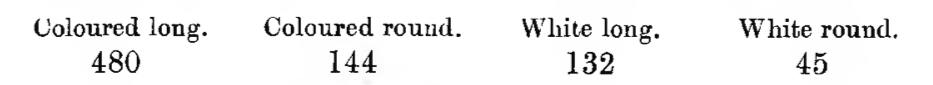
\includegraphics[width=0.8\linewidth]{images/Punnet-page-93} \caption[Figure 2.2]{Figure 2.2: Genetics data from 1905}\label{fig:punnett-93}
\end{figure}

This style of presentation is perfectly understandable, but it is not in the modern format for data. As a data frame, the observations underlying Figure 2.2 would look like Figure 2.3:

\begin{table}

\caption{\label{tab:punnet-raw}Figure 2.3: Punnett's data in a contemporary format}
\centering
\begin{tabular}[t]{l|l|l}
\hline
ID & flower\_color & pollen\_shape\\
\hline
SP2590 & other & long\\
\hline
SP280 & other & long\\
\hline
SP7140 & white & long\\
\hline
SP5260 & other & round\\
\hline
SP7200 & white & long\\
\hline
SP1490 & other & long\\
\hline
\multicolumn{3}{l}{... and so on for 801 rows altogether.}\\
\end{tabular}
\end{table}

You may well wonder what benefit there is to working with an 801-row data frame rather than the simple tabulation in the original publication. First, giving the variables names allows us to distinguish between the variable being measured and the level of the measurement. Second, the table makes clear that both variables \texttt{flower\_color} and \texttt{pollen\_shape} are categorical. Third, suppose there was some other aspect being recorded about the plants, for instance the plant's height or how much water the plant was given or the name of the technician who recorded the data. Using a data frame, these new variables can easily be added as additional columns. There's no space in the tabulation for these additional measurements.

A fourth reason to prefer the data-frame format for the genetics data is subtle. Most often, you will be using software to analyze data. Storing data in a consistent way -- data frames -- makes it much easier to use standard software than if the data are stored in a (pointless) variety of formats.

\hypertarget{quantitative-and-categorical-variables}{%
\section{Quantitative and categorical variables}\label{quantitative-and-categorical-variables}}

The fundamental distinction to be made between types of variables is whether they are quantitative -- a number -- or categorical. Categorical variables are those where the possible values come from a set of discrete categories and are typically represented by text labels.

In the Galton data (Figure 1), height is a quantitative variable. Sex is a categorical variable. The \texttt{family} variable has been encoded as a number, but it is not really numerical. For instance, with numbers, 2 is half way between 1 and 3. But family 2 is not ``between'' families 1 and 2 in any genuinely numerical sense. So \texttt{family} is a categorical variable.

Much later in the book, we will translate categorical variables into a set of very simple numerical variables, each of which is called an \emph{indicator variable}. In an indicator variable, the only allowed values are zero and one.

Obviously, with just zero and one as possible values, a single indicator variable is not able to represent completely a categorical variable with three or more levels. In such situations, a \emph{set of indicator variables} is used. If there are k different levels for the categorical variable, the equivalent set of indicator variables will have k - 1 members. For instance, a variable \texttt{fruit} with three levels ``apple,'' ``blueberry,'' and ``cherry,'' will correspond to two indicator variables. The first one might be whether the fruit is apple or not. The second would be whether the fruit is blueberry or not. When both the first and second take on the value zero, we know that the fruit must be the remaining level, cherry. Figure 5 shows the example on a case by case basis.

\begin{longtable}[]{@{}lcllc@{}}
\toprule
\texttt{fruit} & \(\rightarrow\) & indicator apple & \& & indicator blueberry\tabularnewline
\midrule
\endhead
cherry & & 0 & & 0\tabularnewline
apple & & 1 & & 0\tabularnewline
blueberry & & 0 & & 1\tabularnewline
apple & & 1 & & 0\tabularnewline
cherry & & 0 & & 0\tabularnewline
\bottomrule
\end{longtable}

Figure 5: An example of how a categorical variable (`fruit') can be translated into simple indicator variables. Note that there is always at most a single 1 in each row of the table.

\hypertarget{response-and-explanatory-variables}{%
\section{Response and explanatory variables}\label{response-and-explanatory-variables}}

Starting in Chapter 4, we will work with a standard format for reducing the potentially many rows and variables of a data frame into a single compact object: a \emph{statistical model}. For our purposes, a statistical model will be a \emph{function} that takes inputs and produces an output. In particular, the inputs to each statistical model will be the values of selected variables in the data frame generically called \emph{explanatory variables}. The output of the statistical model will be in terms of the values of a single, selected variable generically called the \emph{response variable}.

The appropriate choice of a response variable and explanatory variables for a model depends on the question that you, the statistical investigator seek to address. Often, to address a broad question, you will use several different statistical models based on the same data frame.

Once you have selected the response and explanatory variables (and a few other details) the process of constructing the corresponding statistical model is a matter of routine calculation, which is always automated. Many people find they can anticipate the results of the calculation for simple models by sketching the graph of a function on a plot of the variables. We delegate the ``oppressive necessity'' of the exact calculations to a computer, leaving our role to give the computer an order: ``Fit the model to the data.''

Keep in mind that response and explanatory variables are not \emph{types} of variables, they are \emph{choices} that we make in building a model. This not withstanding, in this book \emph{all models will have a response variable that is quantitative}. If a categorical variable is to be involved in the response, it will have to be in the form of an indicator variable. On the other hand, explanatory variables can be either quantitative or categorical in any combination.

\hypertarget{measuring-variation}{%
\chapter{Measuring variation}\label{measuring-variation}}

Recall that the purpose of statistical inference is to determine which statistical claims are justified by the data on which they are based. This amounts to asking whether the data provide enough evidence to support a claim. How can we quantify ``how much data is enough?''

An obvious, and important way to quantify ``how much'' is the number of rows in the data frame, that is, the \emph{sample size} \(n\). Perhaps it's intuitive that more data constitutes more evidence. Some care is required here, since we want to avoid phony creation of large sample sizes by copying earlier rows to make new rows in the data frame. A simple way to describe a proper procedure is to insist that each unit of analysis be grabbed at random from the \emph{population} of all the possible units. A data frame constructed by such a procedure is called a \emph{sample of the population}, which is why the number of rows \(n\) is called the sample size.

It's tempting to elaborate on \emph{how much} evidence we have by counting the number of variables in the data frame. But there is a serious problem here. When grabbing a unit from the population, we have a real thing. But there is no such thing as the ``set of possible variables.'' It's the researcher who determines what will be a variable, and you can in principle make up as many as you like. In the running example from Chapter 1, the variables were age and running time. Sensible. But we might also have recorded the runner's favorite number, or the time the runner's brother had breakfast the Tuesday before the race, or anything else, relevant or not. Common sense tells you to avoid such silliness. But what one person considers silly might be sensible to someone else. For instance, many people take seriously astrological signs, but others don't. Should we count astrological sign as a genuine variable? As it happens, birth month accounts for some of the observed differences in performance of professional athletes. (The reason appears to be that children who are the oldest in their school grade do better as kids in athletics, which leads to them developing confidence and interest in sports and receiving extra attention from coaches.)

The key to measuring \emph{how much} evidence the data provides lies in the sentence, ``Birth month accounts for some of the observed differences in performance.'' What matters is whether a variable can \emph{explain} or \emph{account} for the variation in a outcome of interest (like athletic performance). We need to be able to say how much variation there is in the outcome. As described in the previous chapter, in a statistical model the outcome is represented by the response variable. We'll measure the variation in the response variable and then compare it to the amount of variation that the statistical model attributes to the explanatory variable(s).

\hypertarget{variance-of-a-numerical-variable}{%
\section{Variance of a numerical variable}\label{variance-of-a-numerical-variable}}

Recall that the statistical models we use in this book will always have a numerical response variable. We can quantify the amount of variation the response variable in many different ways. The conventional way is by a quantity called the \emph{variance}.

There are different ways to calculate the variance of a variable. Most textbooks give a formula that can be used efficiently by a computer. For the purpose of explaining the variance to another person, I like another way.

The starting point is the response variable for which you want to know the variance. Usually, we organize variables into data frames, but for the moment imagine that the individual numbers, \(n\) of them, have been spilled out on the surface of a table. Take two of the numbers at random. Chances are, the two numbers are different but they might, by luck, be exactly the same. Doesn't matter. To measure the variation of these two numbers, simply subtract one from the other to get the difference, then square the difference. Because of the squaring, it doesn't matter whether you subtract the first number from the second or \emph{vice versa}. For historical reasons, the \emph{variance} is the square difference divided by two. But if history had worked out differently, the square difference would have been a fine measure of variation itself.

The square difference measures the variation between two numbers. But we want to measure the variation of the whole set of numbers. To do this, repeat the calculation of the square difference for \emph{every possible pair of numbers on the table}. For instance, if there were \(n=3\) numbers, say

\[5, 9,  3\]
the pairs would be

\begin{itemize}
\tightlist
\item
  5 - 9 giving a difference of -4 which squares to 16
\item
  5 - 3 giving a difference of 2, which squares to 4
\item
  3 - 9 giving a difference of -6, which squares to 36
\end{itemize}

Now average all the square differences. Averaging 16, 4, 36 gives 18.67. The variance, by historical convention, is half this number, or 9.33.

When \(n\) is big, there are a lot of possible pairs of numbers. For instance, when \(n = 100\), there are 4950 pairs. That's why we leave it to the computer to do the calculation, and even then the calculation is re-arranged so that there are only 100 square differences involved.

If you like, you can think of the reason why we square the difference as a convenience to avoid having to worry about whether the difference is positive or negative (which depends only on which of the pair of values you put first in the subtraction). But there is some profound thinking behind the use of squares, which reflects the nature of randomness and, believe it or not, the Pythagorean theorem.

\hypertarget{variance-of-a-categorical-variable}{%
\section{Variance of a categorical variable}\label{variance-of-a-categorical-variable}}

A categorical variable has distinct \emph{levels}, usually represented by labels such as \emph{agree}, \emph{undecided}, and \emph{disagree}. To describe the amount of variation in a categorical variable we can follow the same process as for numerical variables: spill the collection of \(n\) labels onto a table, pick at random a pair of labels, subtract them, and square the difference.

There's a big problem, however. What is the numerical value of the difference between \emph{agree} and \emph{undecided}? How does the size of the difference between \emph{agree} and \emph{undecided} compare to the difference between \emph{disagree} and \emph{undecided} or between \emph{agree} and \emph{disagree}? Sometimes there's a reasonable choice to be made, for example we might decide that \emph{agree} and \emph{disaggree} differ by 2, \emph{agree} and \emph{undecided} differ by 1, and that \emph{disagree} and \emph{undecided} also differ by 1. Even more basic, it's reasonable to say that the difference between \emph{agree} and \emph{agree} should be zero, and similarly for \emph{disagree} versus \emph{disagree} or \emph{undecided} versus \emph{undecided}.

Notice that all these declared differences can be created by recoding the categorical variable as a numeric variable. For instance, we can change \emph{agree} to 1, \emph{undecided} to 2, and \emph{disagree} to 3. Then just calculate the variance of the numerical variable in the usual way.

Sometimes it's sensible to translate the levels of a categorical variable into numbers. For instance, with \emph{agree}/\emph{undecided}/\emph{disagree} it's reasonable to think that \emph{undecided} is inbetween \emph{agree} and \emph{disagree}. But, in general, there will be no such sense of inbetweenness of categorical levels. Take, for example, a categorical variable whose levels are the names of countries. Or a categorical variable whose levels are political parties: Green, Libertarian, Democratic, Republican. Which levels are between which? (As it happens, people do try to put political parties in sequential order by categorizing them on the scale from Left to Right. This tends to vary between issues, however.)

Without a sense of \emph{inbetweenness} of levels, it's arbitrary to assign numbers to the various levels. Except in one situation.

Often, categorical variables have only two levels. Yes or no. Dead or alive. Accepted or rejected. Treatment and control. Such variables are sometimes called \emph{binary} (like the 0/1 of computer bits) or \emph{dicotomous} or \emph{binomial} (meaning, having two names) or even \emph{two-level}. When dealing with a binary variable, there's no level to be inbetween; there are only two levels and the idea of ``in between'' requires at least three distinct things. So we can easily agree, regardless of our opinions about how the world works, that the difference is zero between labels that are the same (say, \emph{yes} and \emph{yes} or between \emph{no} and \emph{no}). And when the labels are different (say, \emph{yes} and \emph{no}) we just need to assign a non-zero number to the difference.

Which number? Should the square-difference between \emph{yes} and \emph{no} be 17, or 328, or 0.3? By convention, we use the number 1 for the square-difference between the two levels of a binary variable. This convention has the advantage of simplifying calculations. It's also what you will get by treating indicator variables numerically. But there is another important advantage of the simple choice: any average of a 0/1 variable must always be somewhere in the range from 0 to 1, which is exactly the same scale we use for describing \emph{probability}.

The simplicity of dealing with binary variables means that the techniques of statistical inference with a binary categorical response variable are much easier than for non-binary categorical response variables. This is also the most common setting for classical inference. We'll deal with statistical inference on numeric and indicator variables (which are effectively numeric) in this book, leaving questions of inference on non-binary categorical variables for another time.

\hypertarget{modeling-variation}{%
\chapter{Modeling variation}\label{modeling-variation}}

The point of statistics is to understand how things vary. For instance, human height varies from one person to another. Some of that variation is associated with the sex of the person: women \emph{tend to be} slightly shorter than men. Some of the variation in height relates to genes and genetic variation. Some to differing nutrition and general health.

Statistical models attempt to use the variation in explanatory variables -- sex, genetic traits -- to account for the variation in a response variable. To offer a contemporary example, some automobiles are involved in fatal accidents and some (the vast majority, thankfully!) are not. It varies. What's behind the variation? It could be the weather conditions at the time. It could also be human driver fatique, inebriation, incompetence, distraction, etc. It could also be characteristics of the vehicle itself: size, weight, maneuvrability, breaking power, physical wear, automatic breaking, etc. And a lot of the variation is a matter of chance: for instance, the arrival of another car at an intersection at a particular instant.

\hypertarget{statistical-models}{%
\section{Statistical models}\label{statistical-models}}

For our purposes, a statistical model is a mathematical function that takes values of the explanatory variables as input and produces a corresponding output. For instance, a model of a person's height might take the person's age, sex, mother's height and father's height as inputs and give as output a specific number that we interpret as a kind of idealized description of the height of the people who have the same values for those inputs. It might happen, by accident, that the model is exactly on target for any particular person. More likely, though, the model output will be somewhat off: the person is somewhat shorter or taller than the model says. This is to be expected since the model can't take into account every factor that influences height and because chance also plays a role.

\hypertarget{quantitative-response-variables}{%
\section{Quantitative response variables}\label{quantitative-response-variables}}

Consider the model (and data) shown in Figure 4.1. These are Galton's records on the heights of adult children in London families. In Figure 4.1, \texttt{height} has been selected as the response variable. To keep the example simple, the role of explanatory variable has been assigned to \texttt{sex}. The statistical model takes as input a level of \texttt{sex} and produces as output a numerical value for the response variable.

\begin{figure}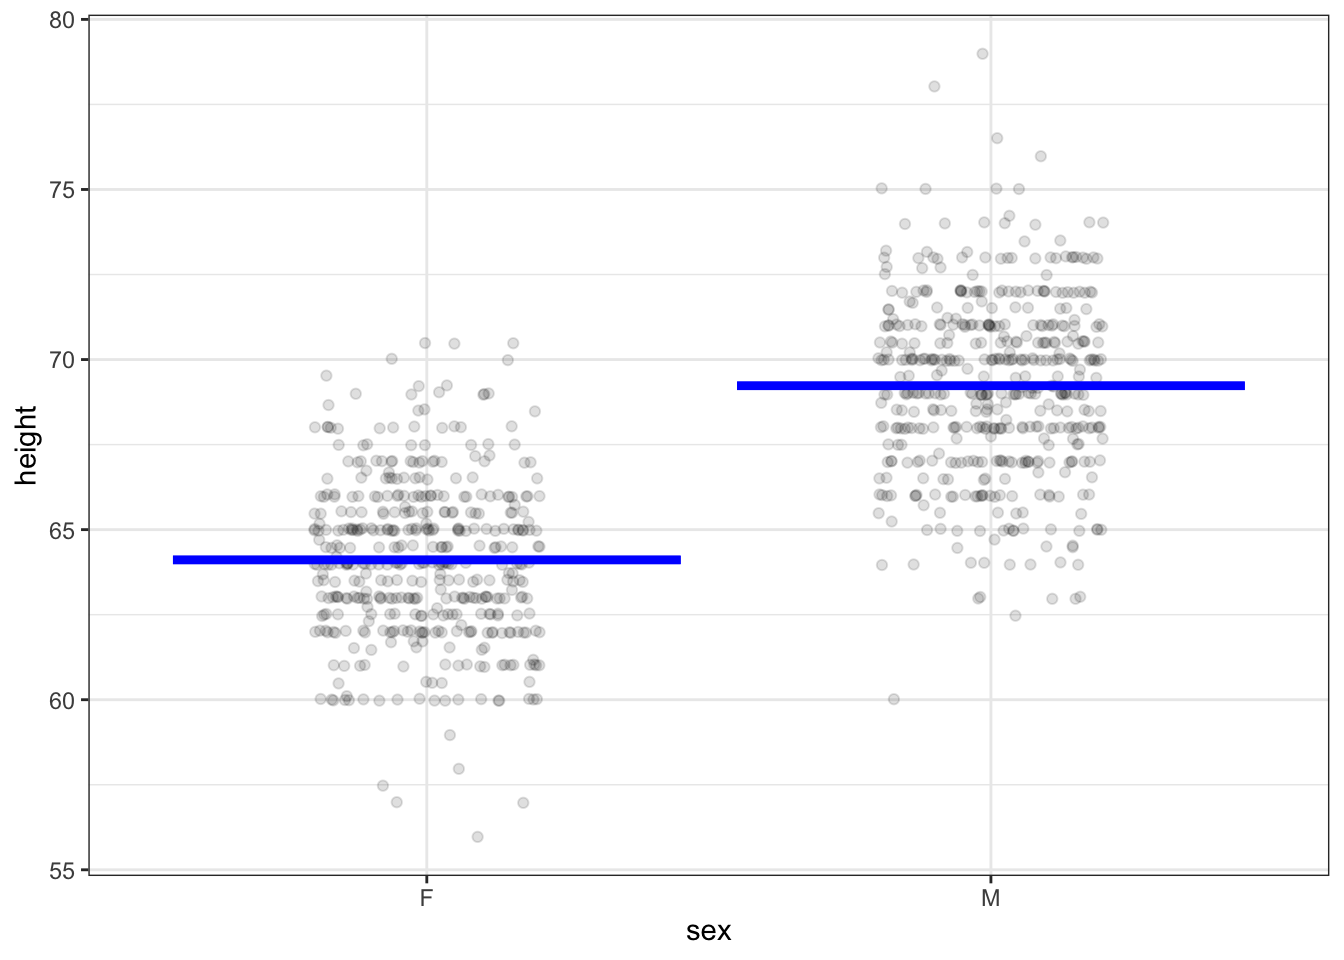
\includegraphics[width=0.8\linewidth]{040-Modeling-Variation_files/figure-latex/galton-0-1} \caption[Figure 4.1]{Figure 4.1: Galton's height measurements with height as the response variable and sex as the explanatory variable. The model gives a single output for each level  of  the explanatory variable.}\label{fig:galton-0}
\end{figure}

As you can see, the output of the model is about 64 inches when sex is F, and 69 inches when sex is M. The preceeding sentence uses stilted language. A straightforward rendering would be something like this: According to the model, women are 64 inches tall and men are 69 inches. But the straightforward account is misleading. While some women are 64 inches tall, the large majority are not, and similarly for men. Neither would it be correct to say that women are shorter than men. Some are and some aren't.

Another mis-statement is that ``the \emph{average} woman is shorter than the \emph{average} man.'' Such language originates in the 1830s, when the idea was that there was an ideal type, from which the the individual might ``deviate.''

If your goal is to describe the relative heights of men and women, better a statement that incorporates the intrinsic variation in height between individuals. For instance, ``The large majority of women fall into the range 60 to 68 inches, while the large majority of men are between 65 and 73 inches tall.''

How were the model outputs determined? Or, in other words, what method was used to construct the model? For now, the details are unimportant. The primary point is that the kind of model being shown describes the \emph{center} of the distribution of individuals. A secondary point is that the model methodology is standard and automatic; the model outputs were established strictly using \texttt{sex} as the explanatory variable without consideration of anything else and without room for a human to manipulate the numbers or shade them into a preferred direction.

The model in Figure 4.1 has an explanatory variable that is categorical. Figure 4.2 is an example where the explanatory variable is numeric. The question that motivated Galton to collect the height data in the first place was to characterize the genetics of height: the extent to which it's fair to say that a child inherits the height of his or her parents.

\begin{figure}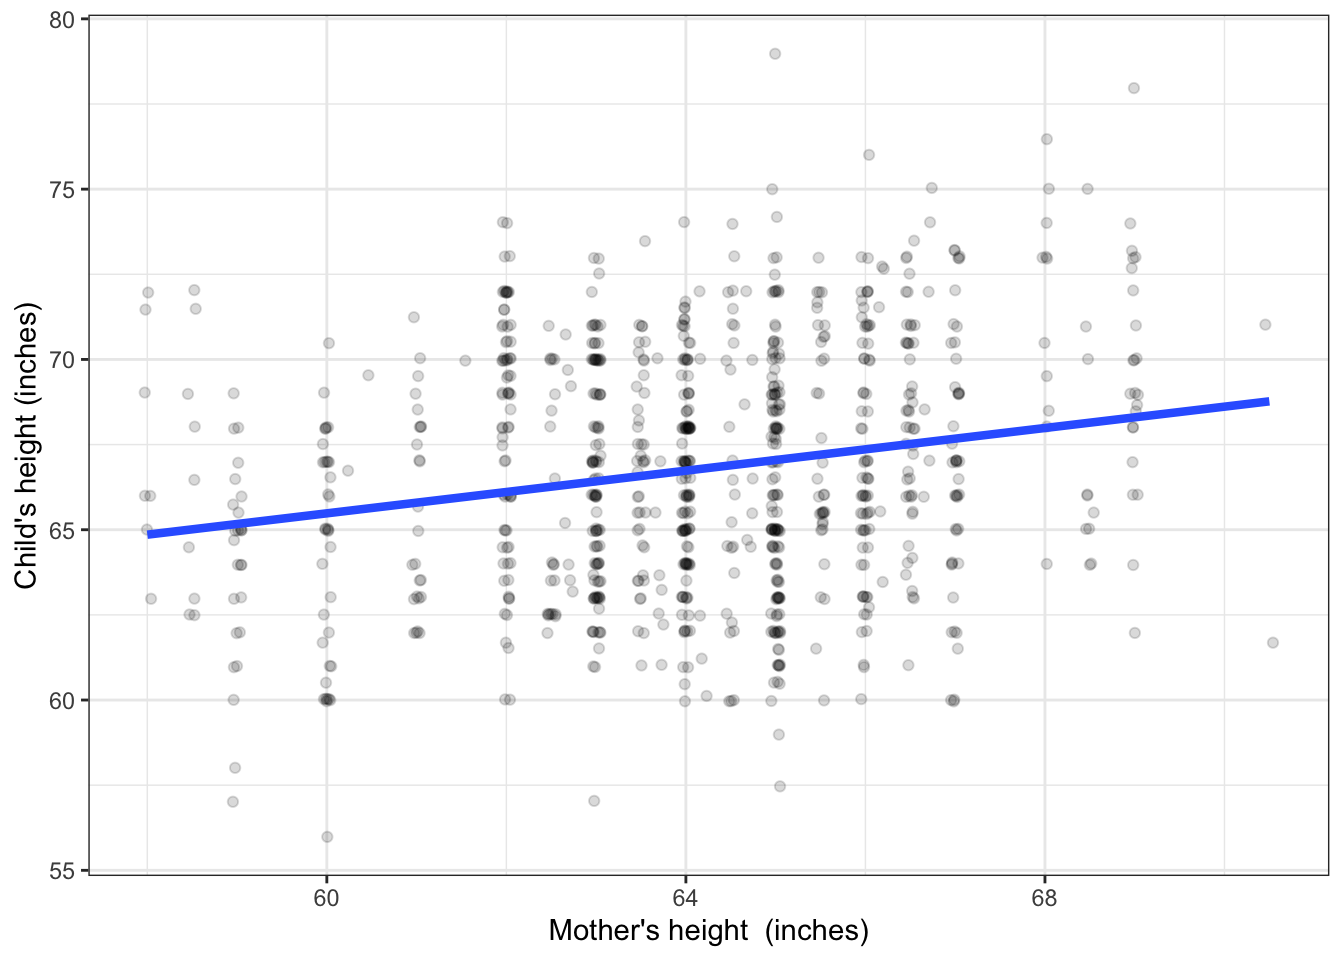
\includegraphics[width=0.8\linewidth]{040-Modeling-Variation_files/figure-latex/galton-2-1} \caption[Figure 4.2]{Figure 4.2:  Child's height versus the mother's height. A conventional form of model is a straight line.}\label{fig:galton-2}
\end{figure}

Consider first the model as a function. The input is the explanatory variable, mother's height. The output is a number. So, for an input of 60 inches, the output is about 66 inches. For an input of 68 inches, the output is somewhat higher: about 68 inches.

The model output discribes the \emph{center} of the distribution of adult-child heights. That center is somewhat lower among the children of relatively short mothers than it is among the children of relatively tall mothers. Note that hardly any individuals match the model output generated at their mother's height; almost all are either shorter or taller.

Some people mistakenly believe that the point of such a model is to \emph{predict} the child's height. Putting aside the question of why anyone would want to do this (perhaps you are wanting to buy a college graduation gown for your pregnant friend's baby?), any meaningful prediction should be framed as an interval. So, for a 60-inch tall mother, a fair prediction would be for a child between 58 and 73 inches, while for a relatively tall 68-inch mother, the prediction would be 62 to 76 inches. What use is that?

Galton's objective in collecting the data was to say \emph{how much} of the variation in height is attributable to genetics. For the record, Figure 2 would be interpreted as the mother's height accounting for about 4\% of the variation in height among children. (Note that it's 4\% of the \emph{variation} in height among children, not 4\% of the height of an individual child.)

Four percent doesn't seem like much. Indeed, looking at Figure 2 and asked to draw a \emph{central} model, you couldn't fault someone for drawing a level line, that is, one where the model output doesn't change at all with mother's height. This is where statistical inference can play an important scientific role. It allows us to detect in a justifiable way very small connections between variables. Key to detecting something small is to avoid false detections: claiming that there is a connection when the data provides little justification. So much of statistical inference has to do with avoiding such false claims.

\hypertarget{proportions-and-indicator-variables}{%
\section{Proportions and indicator variables}\label{proportions-and-indicator-variables}}

The previous examples involved models where the response variable is numeric. This includes an indicator variables used to represent a categorical variable.

Things are particularly straightforward when the categorical response variable has two levels: yes/no, alive/dead, succeed/fail, etc. The reason this is straightforward is that a binary categorical variable can be translated without loss into a single indictor variable.

To illustrate, consider some data from another approach to quantifying genetics by \emph{experimental manipulation}. This tradition started with Gregor Mendel in the 1860s, who famously cross bred peas. Students of genetics know the name Mendel. Another famous name is Reginald Punnett (as in the Punnett square), whose cross-breeding work was done around 1905.

In one experiment, Punnett cross bred sweet peas and observed the flower color (binary levels white/other) and the shape of pollen granules (binary levels round/long). A few rows of data (translated to a modern format) from this experiment are shown in Figure 1.4 in Chapter 1. The complete data are graphed in Figure 4.3, below.

\begin{figure}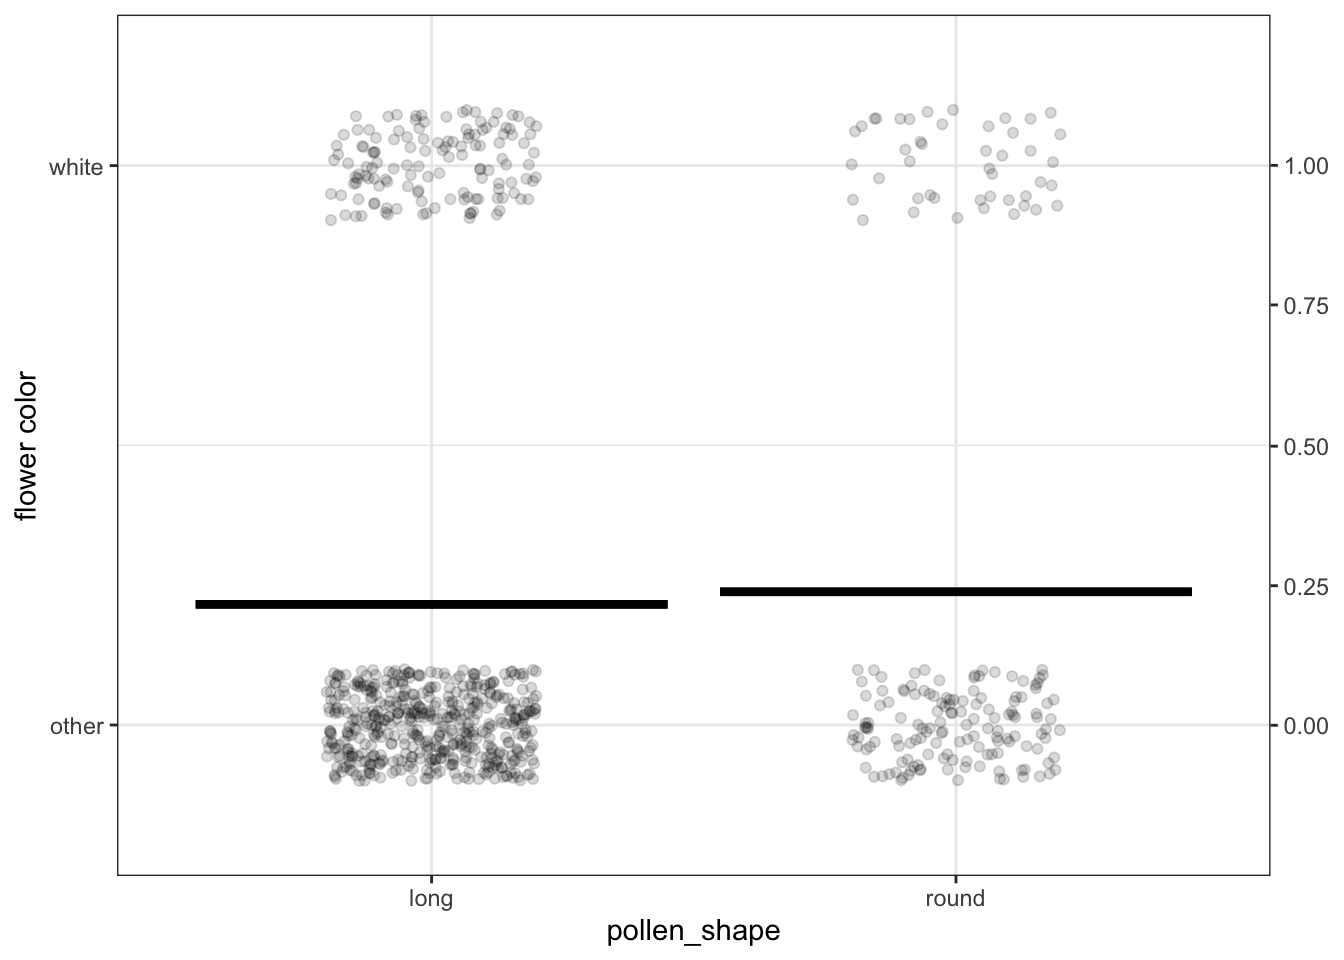
\includegraphics[width=0.8\linewidth]{040-Modeling-Variation_files/figure-latex/punnett-1-1} \caption[Figure 4.3]{Figure 4.3: Punnett's data from cross breeding peas, along with a model of flower color versus pollen shape.}\label{fig:punnett-1}
\end{figure}

There are only four possible combinations of white/other and long/round. To avoid plotting the rows directly on top of one another, the dots have been \emph{jittered}. You can see that peas with ``other'' color and long pollen grains are the most common.

The model here is very similar to that of Figure 4.1. The response variable, flower color, has been translated into an indicator variable taking on only the values zero or one. The model provides an output for each level of the explanatory variable, pollen shape. Notice that the model output is not set in terms of white/other, but as a number. The model output is usually interpreted as a probability. For instance, when the pollen shape is long, the model output is just under 0.25, meaning that about a quarter of the plants had white flowers. When the pollen is round, the model value is a little heigher but not much. Again about a quarter of the plants with round pollen had white flowers. (Is the claim justified by the data that the probability is higher for round-pollen plants than for long-pollen plants? Statistical inference provides an answer to this question.)

You can pretty much draw functions like this by hand. Mathematically, though, there are some restrictions. First, the function has to stay as close to the data as possible. Second, the function has to stay centered on the data. (Technically, the function form has to include an intercept.) It might be easiest to understand these restrictions by looking at some crazy bad functions that don't honor the restrictions, like the one in Figure 4.3.

\begin{figure}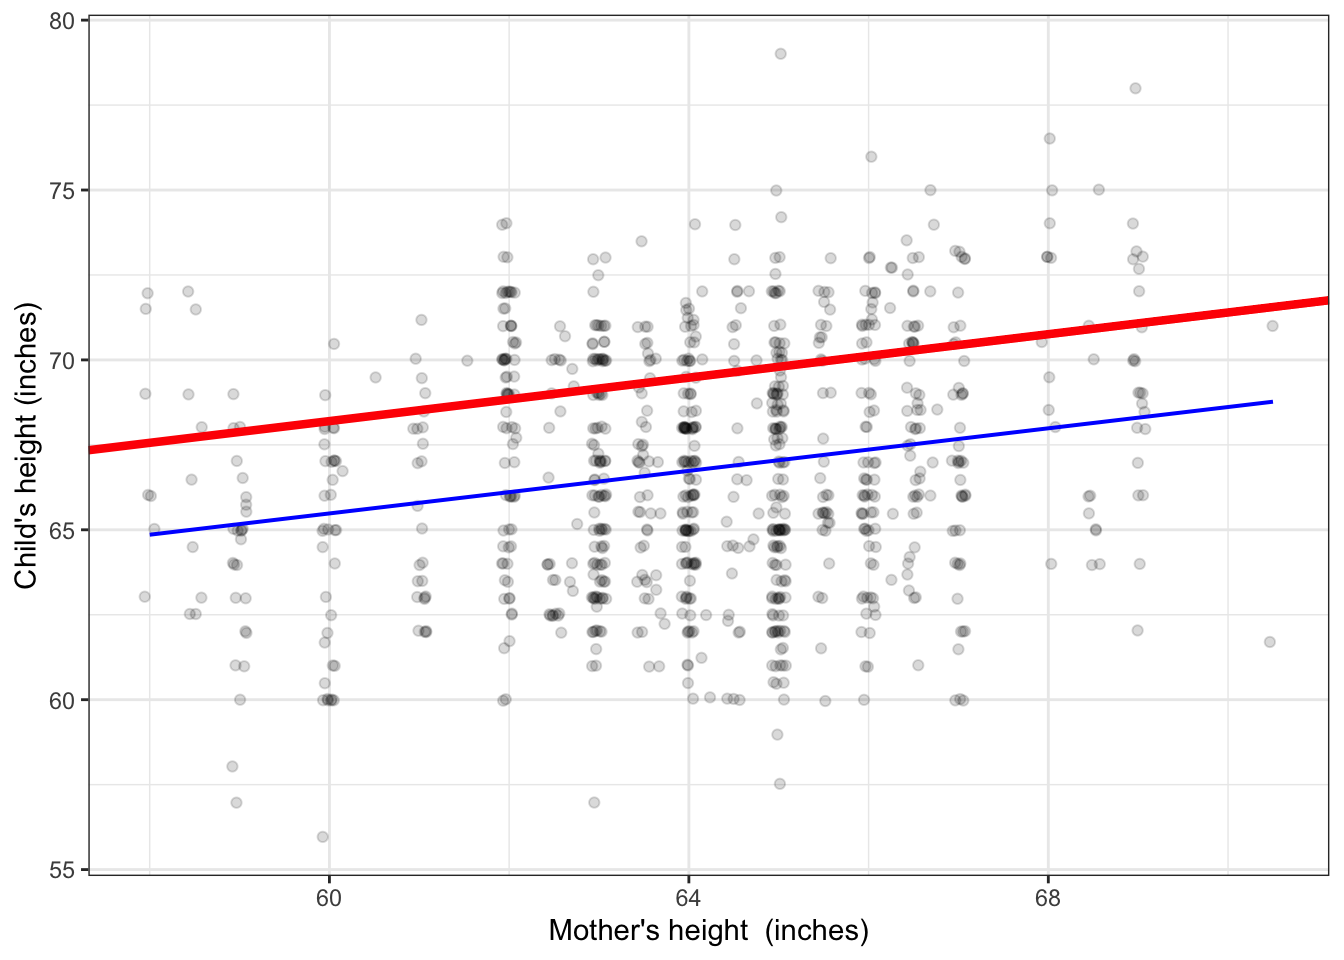
\includegraphics[width=0.8\linewidth]{040-Modeling-Variation_files/figure-latex/fig-4-3-1} \caption[Figure 4.3]{Figure 4.3: The function in red is a bad match to the data. It strays from the data at the extremes. The blue function has the same form -- a straight line -- but is a legitimate match to the data.}\label{fig:fig-4-31}
\end{figure}
\begin{figure}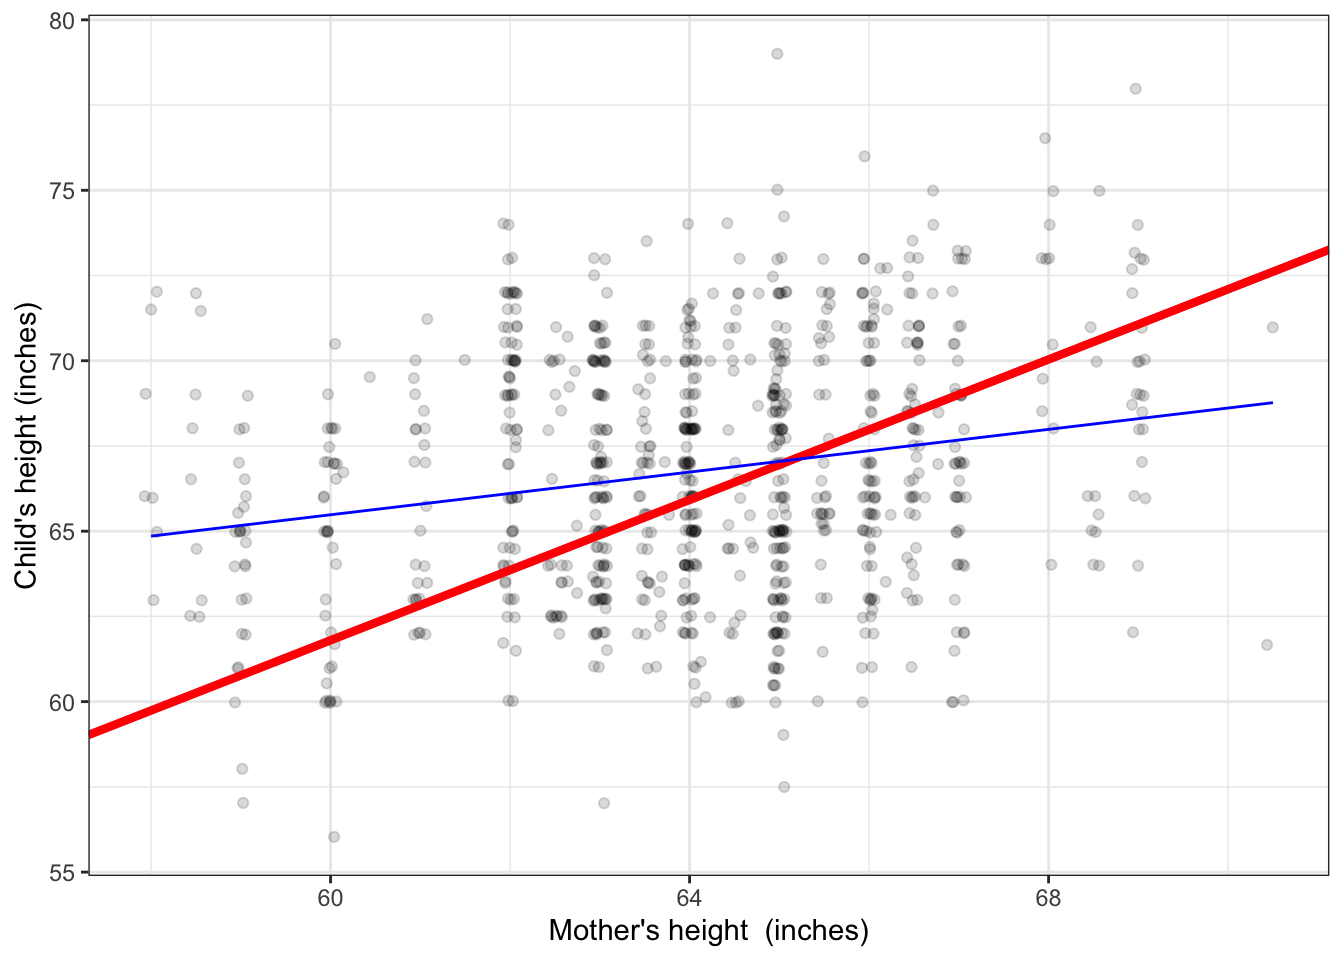
\includegraphics[width=0.8\linewidth]{040-Modeling-Variation_files/figure-latex/fig-4-3-2} \caption[Figure 4.3]{Figure 4.3: The function in red is a bad match to the data. It strays from the data at the extremes. The blue function has the same form -- a straight line -- but is a legitimate match to the data.}\label{fig:fig-4-32}
\end{figure}

Note that the blue functions in Figure 4.3 are centered in the sense that whatever value for the explanatory variable you look at, the data points are just about evenly distributed above and below the function. The red functions don't accomplish this.

The previous examples have all involved a response variable and a \emph{single} explanatory variable. Since variables can be either numerical or quantitative, logic suggests there are four possible settings for models, of which we've seen three. Figure 4.4 shows the fourth setting, a categorical response variable and a numerical explanatory variable.

\begin{figure}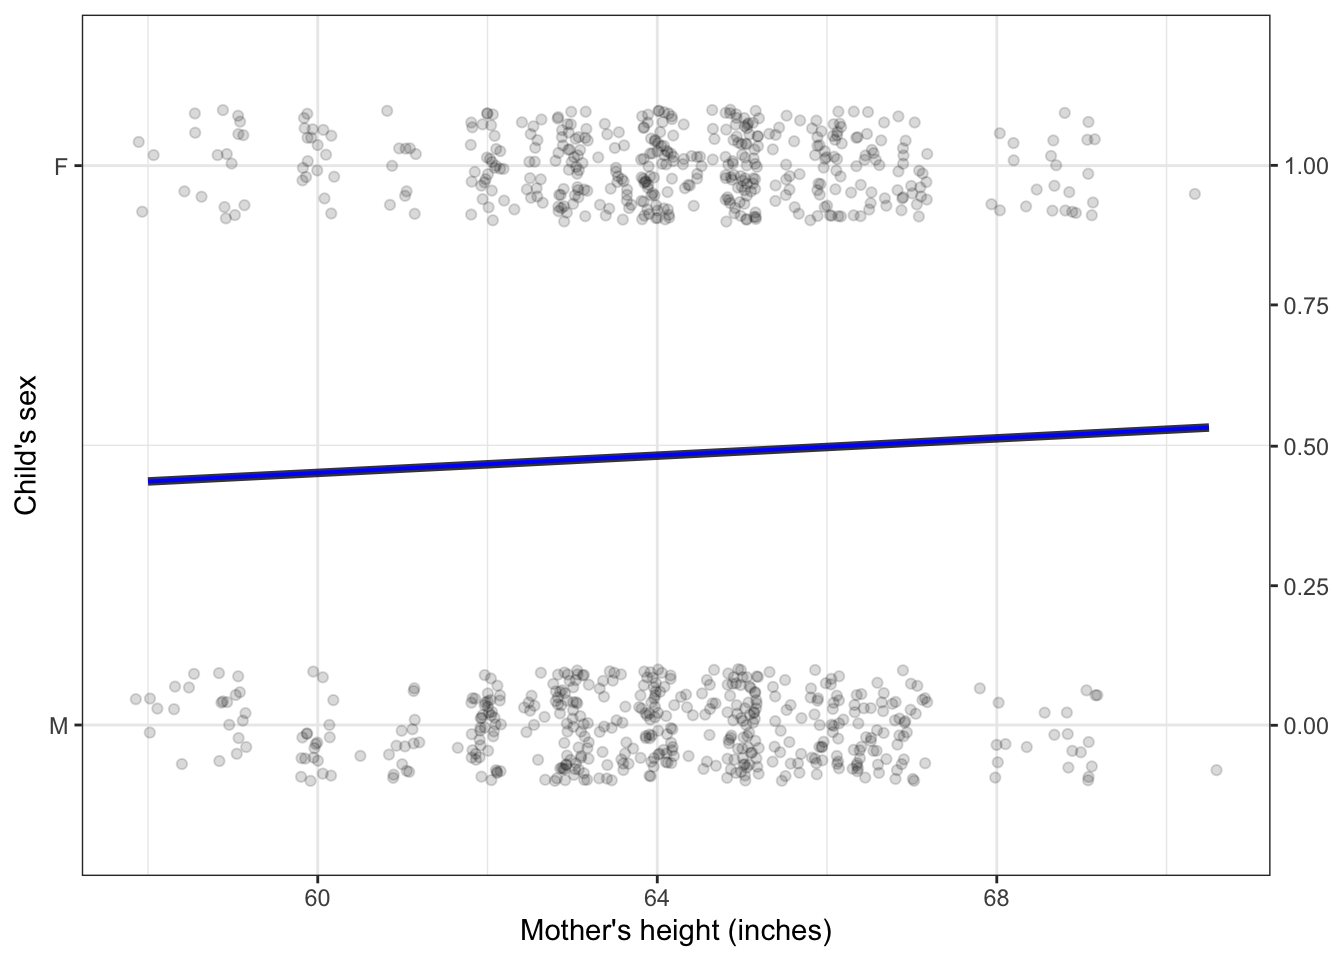
\includegraphics[width=0.8\linewidth]{040-Modeling-Variation_files/figure-latex/galton-logistic-1} \caption[Figure 4.4]{Figure 4.4: A model with a binary categorical response variable and a numerical explanatory variable.}\label{fig:galton-logistic}
\end{figure}

Again, the model output is numeric, in the form of the probability that the child is female. The model suggests that 60-inch tall mothers are slightly less likely to bear girls and 68-inch tall mothers. As you might expect, the model output is around 50\% regardless of the mother's height.

Perhaps you're surprised to see that the mother's height is related to the sex of the baby. Don't be surprised yet, because we haven't shown that such a statement is justified by the data: we have a setting for inference but have not yet carried out the inference calculations to tell us if the statement is justified.

In this section, I've sketched out four settings for statistical modeling with different combinations of categorical/numeric for the response and explanatory variables. In all settings, exactly the same technique, called \emph{linear regression}, has been used to match the model to the data. I'll summarize this with a table that shows the four combinations and refers you to the corresponding table.

\begin{longtable}[]{@{}lllll@{}}
\toprule
\begin{minipage}[b]{0.03\columnwidth}\raggedright
~\strut
\end{minipage} & \begin{minipage}[b]{0.24\columnwidth}\raggedright
response var\strut
\end{minipage} & \begin{minipage}[b]{0.29\columnwidth}\raggedright
explanatory var\strut
\end{minipage} & \begin{minipage}[b]{0.15\columnwidth}\raggedright
Figure\strut
\end{minipage} & \begin{minipage}[b]{0.14\columnwidth}\raggedright
conventional name\strut
\end{minipage}\tabularnewline
\midrule
\endhead
\begin{minipage}[t]{0.03\columnwidth}\raggedright
1\strut
\end{minipage} & \begin{minipage}[t]{0.24\columnwidth}\raggedright
quantitative\strut
\end{minipage} & \begin{minipage}[t]{0.29\columnwidth}\raggedright
categorical\strut
\end{minipage} & \begin{minipage}[t]{0.15\columnwidth}\raggedright
4.1\strut
\end{minipage} & \begin{minipage}[t]{0.14\columnwidth}\raggedright
groupwise means / t-test\strut
\end{minipage}\tabularnewline
\begin{minipage}[t]{0.03\columnwidth}\raggedright
2\strut
\end{minipage} & \begin{minipage}[t]{0.24\columnwidth}\raggedright
quantitative\strut
\end{minipage} & \begin{minipage}[t]{0.29\columnwidth}\raggedright
quantitative\strut
\end{minipage} & \begin{minipage}[t]{0.15\columnwidth}\raggedright
4.2\strut
\end{minipage} & \begin{minipage}[t]{0.14\columnwidth}\raggedright
linear regression / slope test\strut
\end{minipage}\tabularnewline
\begin{minipage}[t]{0.03\columnwidth}\raggedright
3\strut
\end{minipage} & \begin{minipage}[t]{0.24\columnwidth}\raggedright
categorical (indicator)\strut
\end{minipage} & \begin{minipage}[t]{0.29\columnwidth}\raggedright
categorical\strut
\end{minipage} & \begin{minipage}[t]{0.15\columnwidth}\raggedright
4.3\strut
\end{minipage} & \begin{minipage}[t]{0.14\columnwidth}\raggedright
groupwise proportions / p-test\strut
\end{minipage}\tabularnewline
\begin{minipage}[t]{0.03\columnwidth}\raggedright
4\strut
\end{minipage} & \begin{minipage}[t]{0.24\columnwidth}\raggedright
categorical (indicator)\strut
\end{minipage} & \begin{minipage}[t]{0.29\columnwidth}\raggedright
quantitative\strut
\end{minipage} & \begin{minipage}[t]{0.15\columnwidth}\raggedright
4.4\strut
\end{minipage} & \begin{minipage}[t]{0.14\columnwidth}\raggedright
not usually included in introductory statistics\strut
\end{minipage}\tabularnewline
\bottomrule
\end{longtable}

Recognizing that many readers have studied statistics before, I've added to the table the conventional name assigned to the inferential test in that setting in introductory statistics. Also, for the conventionally-trained reader, I acknowledge that the term \emph{linear regression} is conventionally applied only to setting 2. But there is no good reason for this: all four settings can be handled with exactly the same modeling process.

\hypertarget{model-values}{%
\chapter{Model values}\label{model-values}}

It's now time to talk a bit about the way that statistical models are constructed. To do this, imagine that we have a classroom full of students, each of whom is given data in the form of the graphs of the previous chapter and asked to draw a straight-line function relating the explanatory variable to the response variable. Naturally, some students' models will be better than others. How can we determine which model is the best?

To illustrate, let's take a small data set and look at two models that students might draw. (Figure 5.1)



\begin{figure}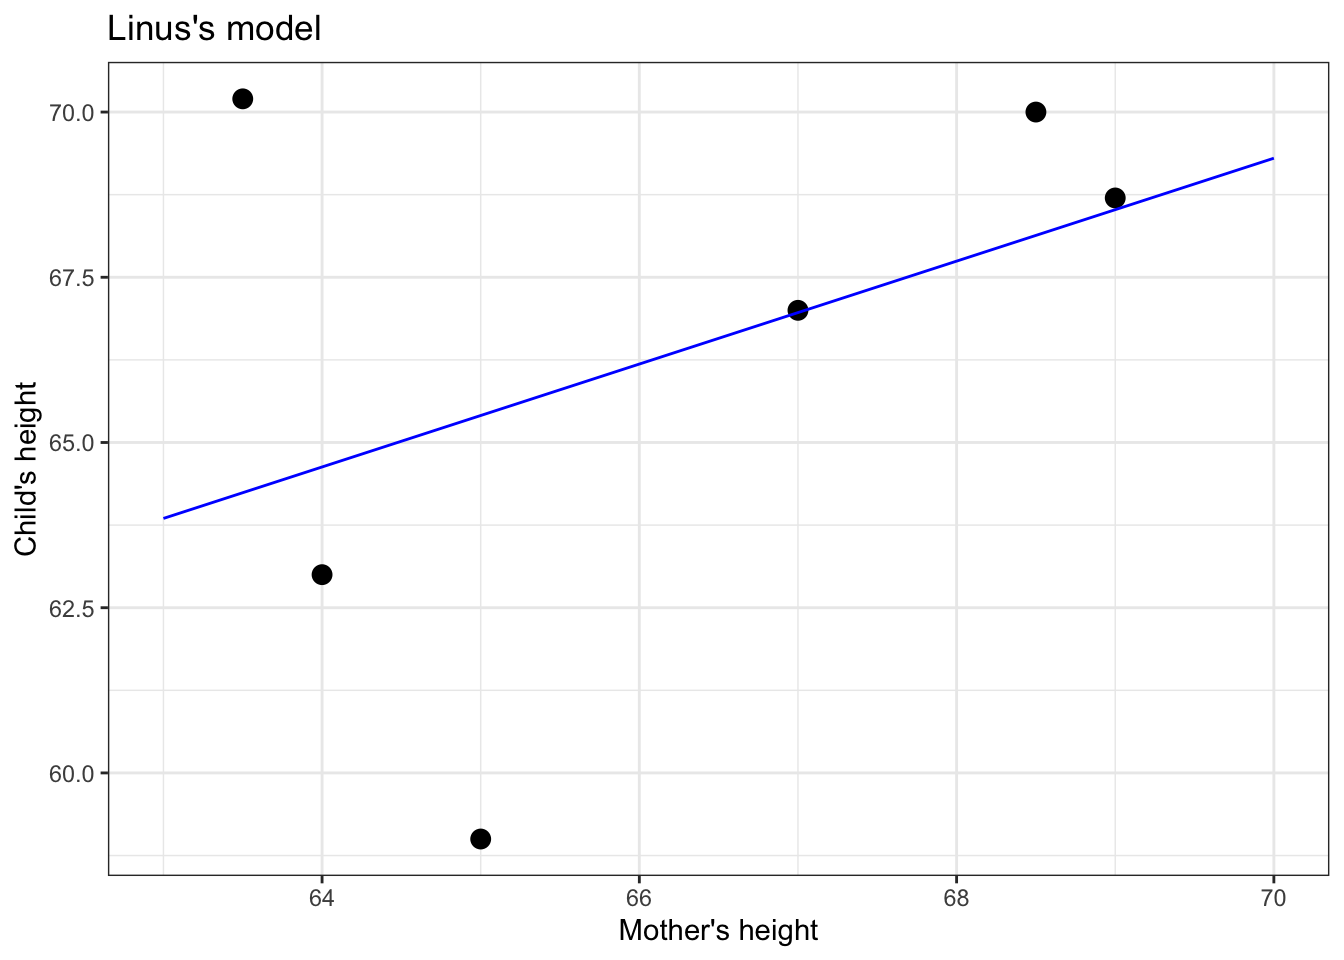
\includegraphics[width=0.5\linewidth]{043-Model-values_files/figure-latex/drawn-train-1} \caption[Figure 5.1: Comparing two possible straight-line models. In constructing a model, we choose the candidate with the least error.]{Figure 5.1: Comparing two possible straight-line models. In constructing a model, we choose the candidate with the least error.}\label{fig:drawn-train}
\end{figure}
\begin{figure}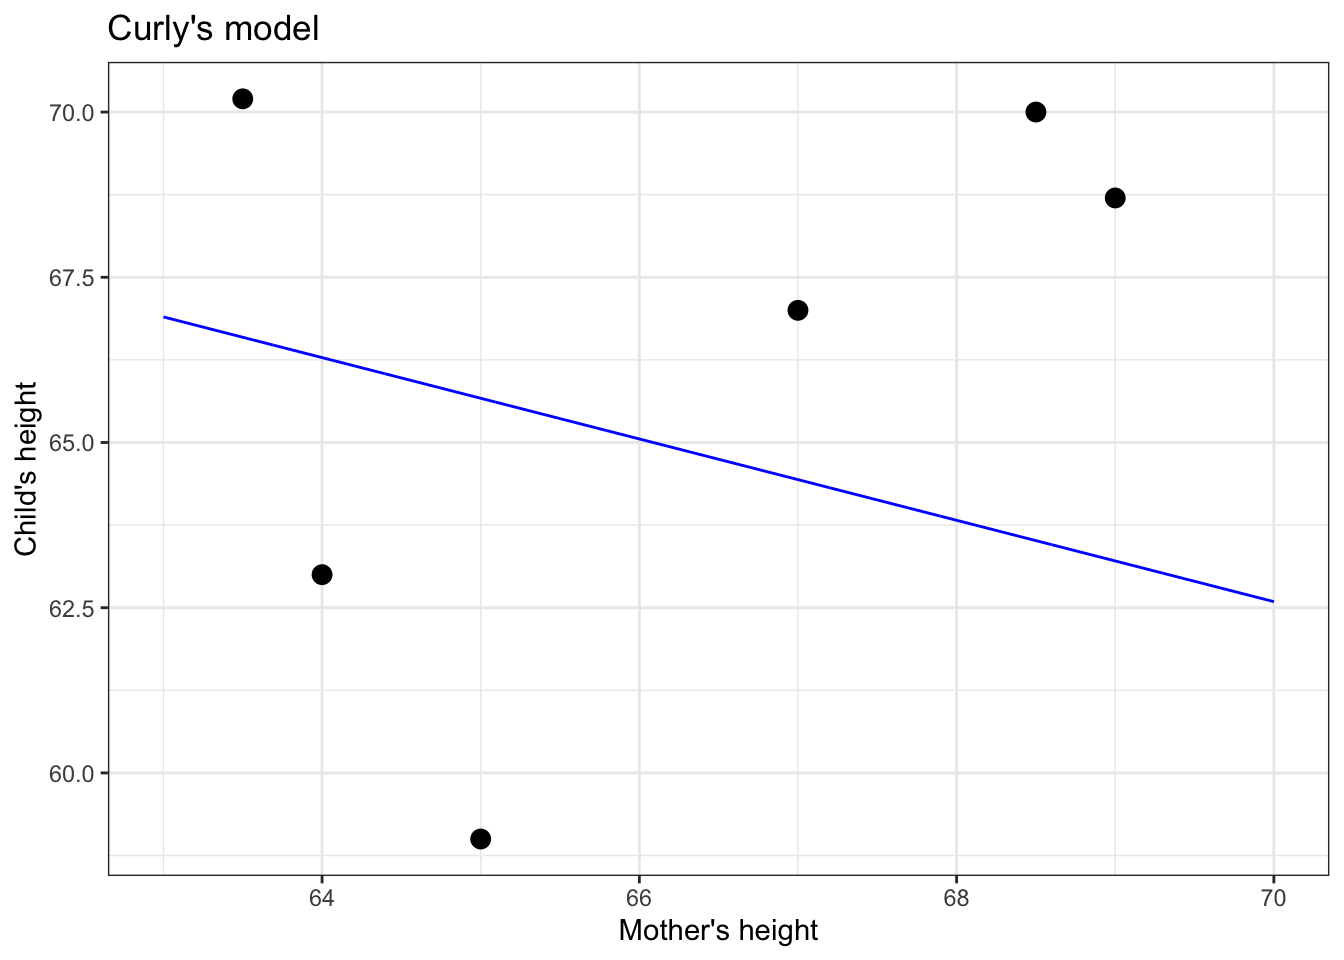
\includegraphics[width=0.5\linewidth]{043-Model-values_files/figure-latex/drawn-train-2} \caption[Figure 5.1: Comparing two possible straight-line models. In constructing a model, we choose the candidate with the least error.]{Figure 5.1: Comparing two possible straight-line models. In constructing a model, we choose the candidate with the least error.}\label{fig:drawn-train}
\end{figure}

Who has drawn the better model: Linus or Curly? The instructor takes out a blue pen and draws a * for every data point. The star marks the output of the model when given the input (mother's height) for that point. The position of each * on the vertical axis marks the \emph{model value} for that data point.

Think of the model values as a kind of stand-in for the response variable, one that stays strictly in line with the model.

Now, the instructor takes out her red pen to mark the ``error.'' The error is the difference between the value of the response variable (black dot) and the model value. The less red ink, the better. Linus wins.

This is analogous to how statistical models are constructed. Once the explanatory and response variables have been selected, and a shape for the function chosen (here, a straight line), the computer tries out all the possibilities and picks the one that gives the least error between the \emph{model values} and the actual response values.

In practice, for straight-line models (and more general forms, called ``linear models''), there are equations that can be solved to find the best model, so there's no need for the computer to try out lots of candidates. But the result is no different than if it had been found by trial and error.

There is something important to notice about the model values for the winning model:

\begin{quote}
\emph{Model values will have a lower variance than the response variable.}
\end{quote}

We'll use the symbol \(v_m\) to stand for the variance of the model values.

To illustrate this, let's look at a couple of models from the previous chapter. In each, you can see that the response values (black dots) are spread out, while the model values stay in toward the center of data. This is a natural consequence of our using \emph{central} models, that is, models where the function has roughly equal numbers of data points above it and below it.

\begin{figure}\includegraphics[width=0.8\linewidth]{043-Model-values_files/figure-latex/unnamed-chunk-2-1} \caption[Figure 5.2: Model values (blue dots) for a straight-line model of child's height with mother's height as the explanatory variable. Response variance: 12.84; Model value variance: 0.52]{Figure 5.2: Model values (blue dots) for a straight-line model of child's height with mother's height as the explanatory variable. Response variance: 12.84; Model value variance: 0.52}\label{fig:unnamed-chunk-2}
\end{figure}



\begin{figure}\includegraphics[width=0.8\linewidth]{043-Model-values_files/figure-latex/unnamed-chunk-3-1} \caption[Figure 5.3: Model values for the probability that a pea has a flower colored white, with pollen shape as the explanatory variable. Response variance: 0.17; Model value variance: 0.000091]{Figure 5.3: Model values for the probability that a pea has a flower colored white, with pollen shape as the explanatory variable. Response variance: 0.17; Model value variance: 0.000091}\label{fig:unnamed-chunk-3}
\end{figure}



\begin{figure}\includegraphics[width=0.8\linewidth]{043-Model-values_files/figure-latex/unnamed-chunk-4-1} \caption[Figure 5.4: Model values for a model of sex, with mother's height as the explanatory variable. Response variance: 0.25; Model value variance: 0.14]{Figure 5.4: Model values for a model of sex, with mother's height as the explanatory variable. Response variance: 0.25; Model value variance: 0.14}\label{fig:unnamed-chunk-4}
\end{figure}



\hypertarget{degrees-of-flexibility}{%
\chapter{Degrees of flexibility}\label{degrees-of-flexibility}}

Chapter 4 introduced four different \emph{settings} for models. (For easy reference, Figure 1 redraws the examples from Chapter 4.) Remember that the word ``settings'' is \emph{not} about the situation that produced the data or the names of the variables being displayed. ``Settings'' refers to the kind of response variable and explanatory variable -- categorical or numerical -- begin used in the model.

This chapter introduces some important new settings:

\begin{itemize}
\tightlist
\item
  Settings with more than one explanatory variable
\item
  Settings where a categorical explanatory variable has more than two levels.
\item
  Settings where the straight-line functions seen in Figure 1(b) and 1(d) are replaced with more flexible curves.
\end{itemize}

It's far from obvious, but these new kinds of settings are all the same kind of thing mathematically, so statistical inference can handle them in the same way. The central concept that links the new settings is called the \emph{degrees of flexibility}.

\hypertarget{one-degree-of-flexibility}{%
\section{One degree of flexibility}\label{one-degree-of-flexibility}}

Each of the models presented in Chapter 4 has a single \emph{degree of flexibility}, that is, \(df = 1\). One way to think about degrees of flexibility is how many numbers are required to specify the model completely. For instance, the straight-line models in Figure 1(b) and 1(d) each can be specified by a \emph{slope} and an \emph{intercept}. The models in Figure 1(a) and 1(b) can be specified by two numbers: the value of the model for the left group and the value for the right group.



\begin{figure}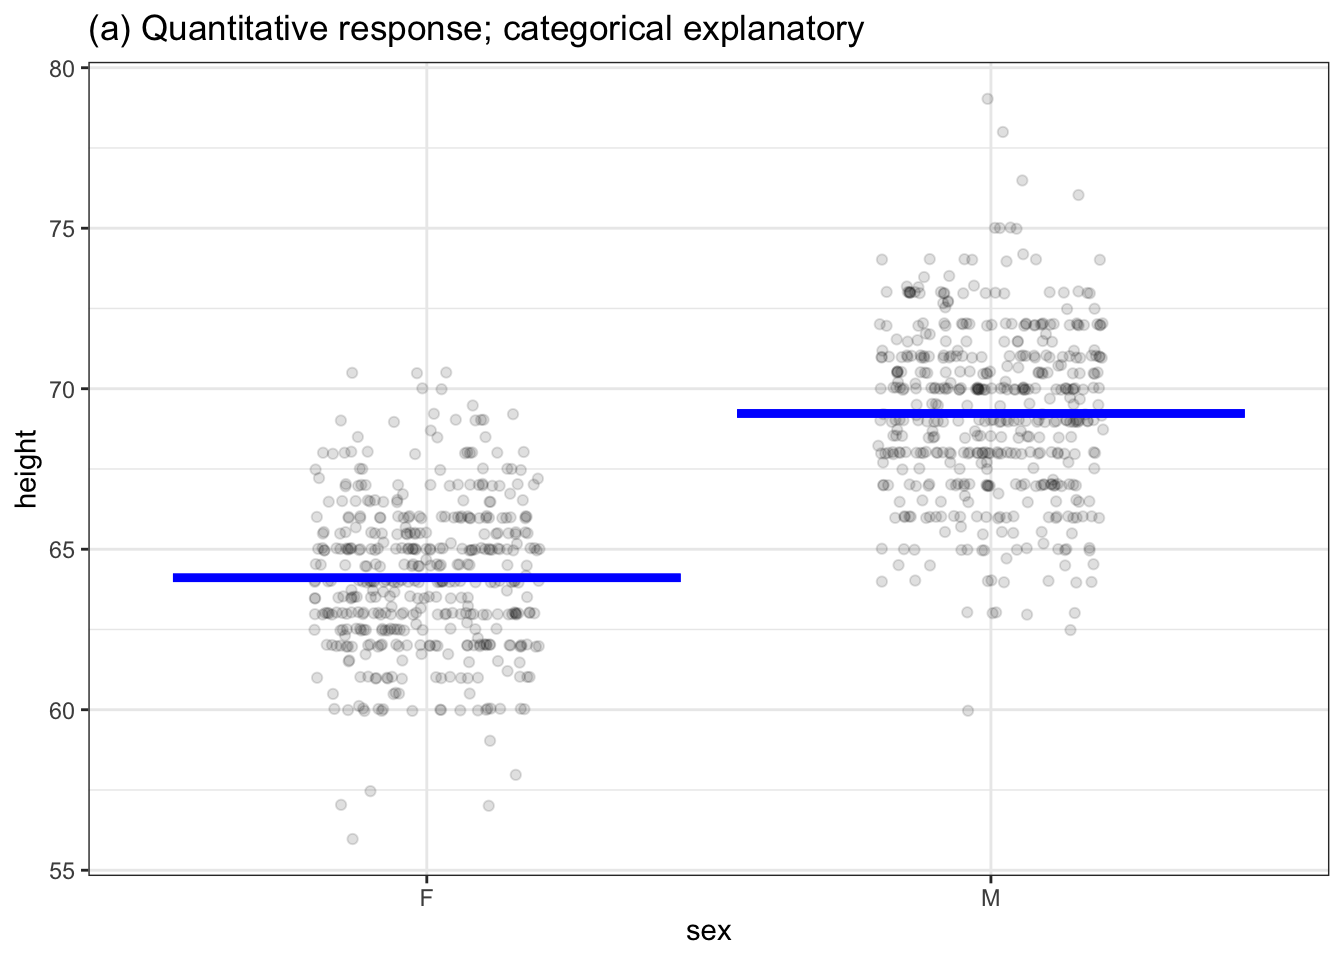
\includegraphics[width=0.5\linewidth]{045-Multiple-explanatory_files/figure-latex/four-settings-1} \caption[(ref:four-settings-cap]{(ref:four-settings-cap}\label{fig:four-settings}
\end{figure}
\begin{figure}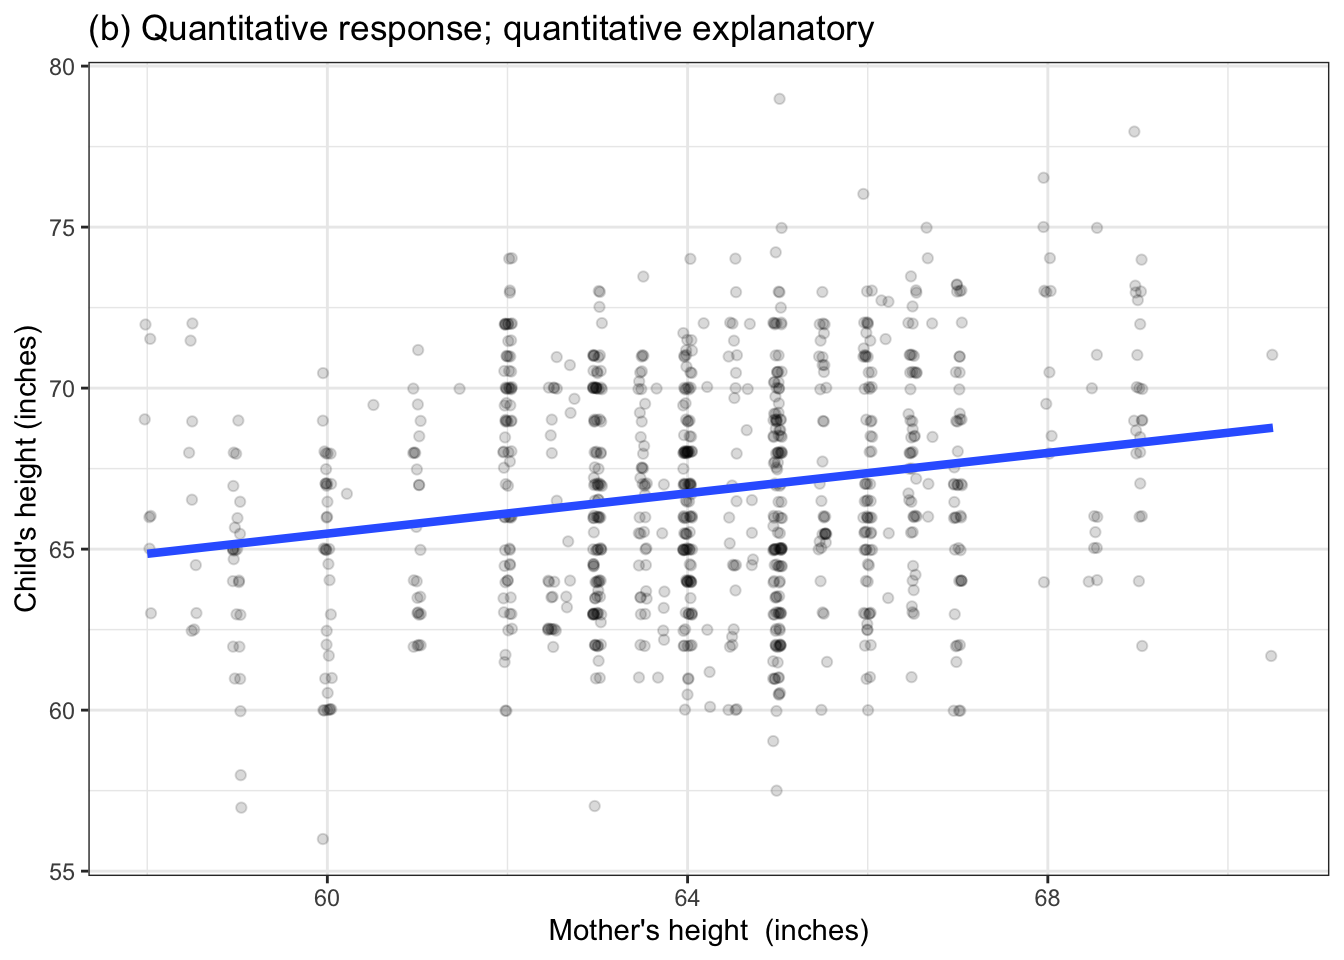
\includegraphics[width=0.5\linewidth]{045-Multiple-explanatory_files/figure-latex/four-settings-2} \caption[(ref:four-settings-cap]{(ref:four-settings-cap}\label{fig:four-settings}
\end{figure}
\begin{figure}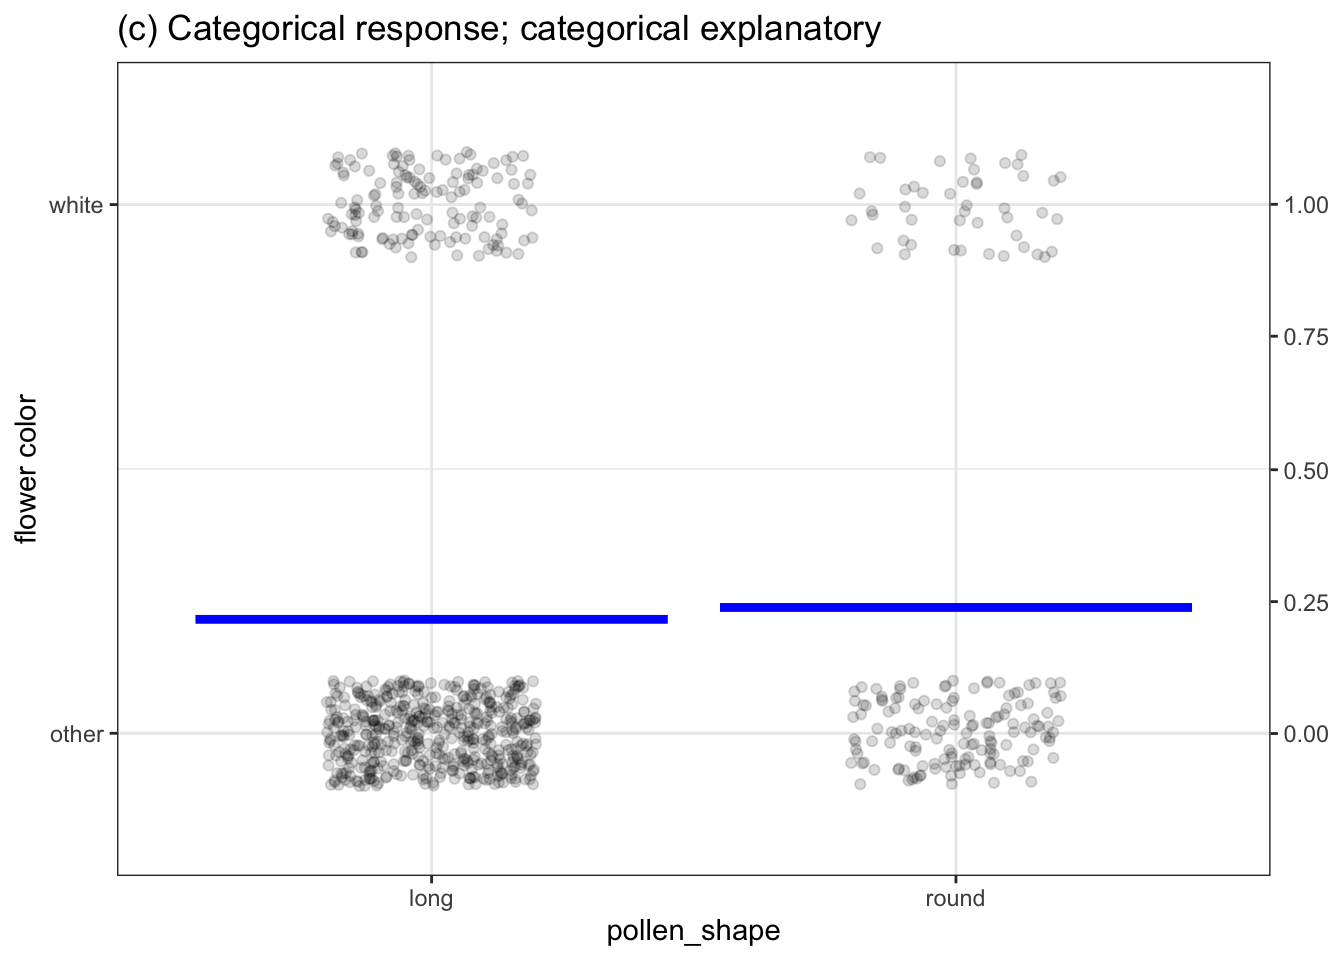
\includegraphics[width=0.5\linewidth]{045-Multiple-explanatory_files/figure-latex/four-settings-3} \caption[(ref:four-settings-cap]{(ref:four-settings-cap}\label{fig:four-settings}
\end{figure}
\begin{figure}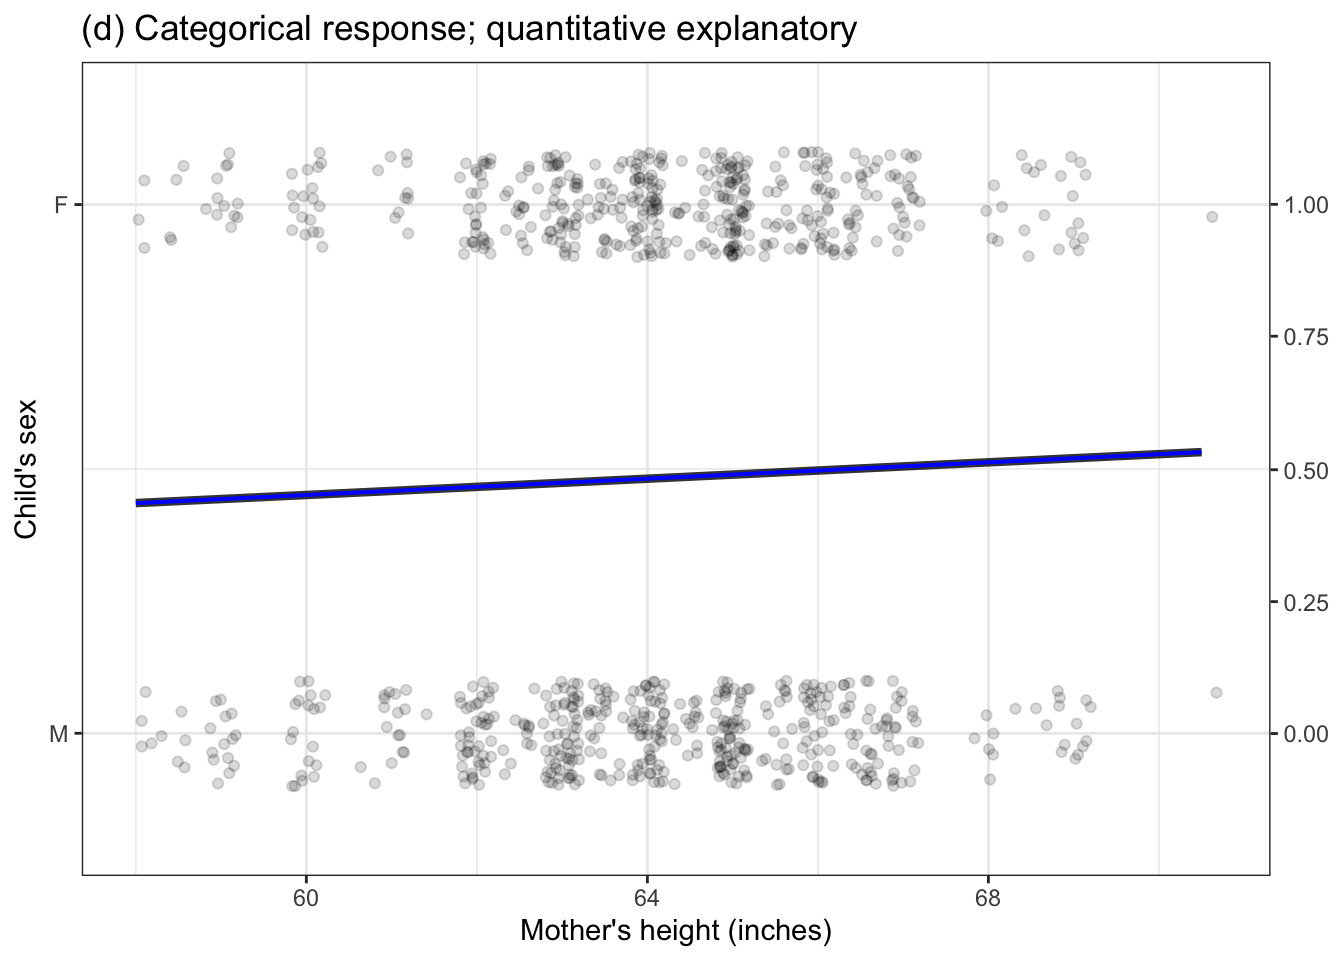
\includegraphics[width=0.5\linewidth]{045-Multiple-explanatory_files/figure-latex/four-settings-4} \caption[(ref:four-settings-cap]{(ref:four-settings-cap}\label{fig:four-settings}
\end{figure}

In talking about descriptions of models, rather than using the word \emph{number}, we use \emph{coefficient}. This is no big deal, but when you see the word \emph{coefficient} you'll have a distinct hint that we are talking about the shape of a model. And we'll be able to say things like ``the \emph{number} of \emph{coefficients}'' to refer to how many coefficients are needed to specify the model.

The degree of flexibility of a model is defined to be the number of coefficients needed to completely specify the model \emph{minus one}. You might wonder, ``Why subtract one from the number of coefficients?'' Just a convention. You'll see some justification for it in Chapter 8, \emph{Simple means and proportions}, where we will work with models with \emph{zero degrees of freedom}, which is to say, one coefficient.

\hypertarget{multiple-degrees-of-flexibility}{%
\section{Multiple degrees of flexibility}\label{multiple-degrees-of-flexibility}}

Let's look at some examples of models where there is more than one degree of freedom. To start, Figure 2 shows a model with two degrees of freedom.

\begin{figure}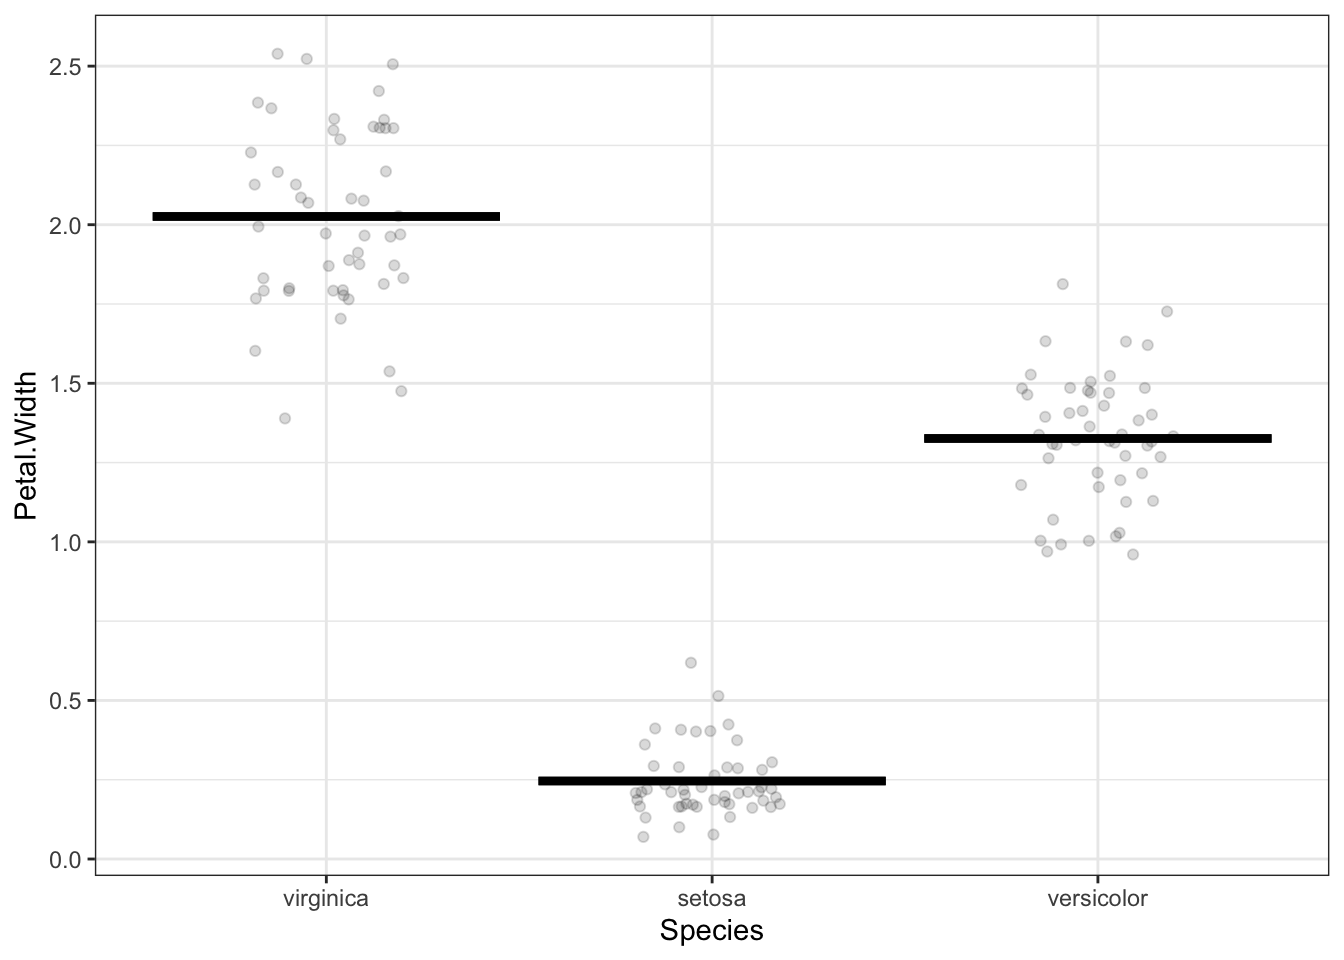
\includegraphics[width=0.8\linewidth]{045-Multiple-explanatory_files/figure-latex/two-df-1} \caption[(ref:two-df-cap)]{(ref:two-df-cap)}\label{fig:two-df}
\end{figure}

The data in Figure 2 are from a classic study involving the differences and similarities among three species of iris plants. The response variable is the flower petal width (quantitative) and the explanatory variable is the species of the plant (categorical). A complete description of the model would involve three coefficients, one for each of the species of iris. Three coefficients corresponds to \(df = 2\).

If the explanatory variable had four levels, there would be \(df=3\), and so on.

There's just a single explanatory variable in Figure 2 (albeit one with three categorical levels). Many models have more than one explanatory variable. Figure 3 shows an example, where the response variable is height and bother mother's height and child's sex are being used as explanatory variables.

The model in Figure 3 consists of two straight lines. Each line is specified by a slope and an intercept, meaning that four coefficients are needed. Thus, \(df=3\).

You may notice that the two lines in Figure 3 have slightly different slopes. Often, modelers try to economize with degrees of flexibility by using the same slope for each line. This would reduce the degrees of freedom to \(df = 2\). (The decision of whether to use a common slope or two potentially different slopes is often made using the tools of statistical inference, but we are getting ahead of the story.)

\begin{figure}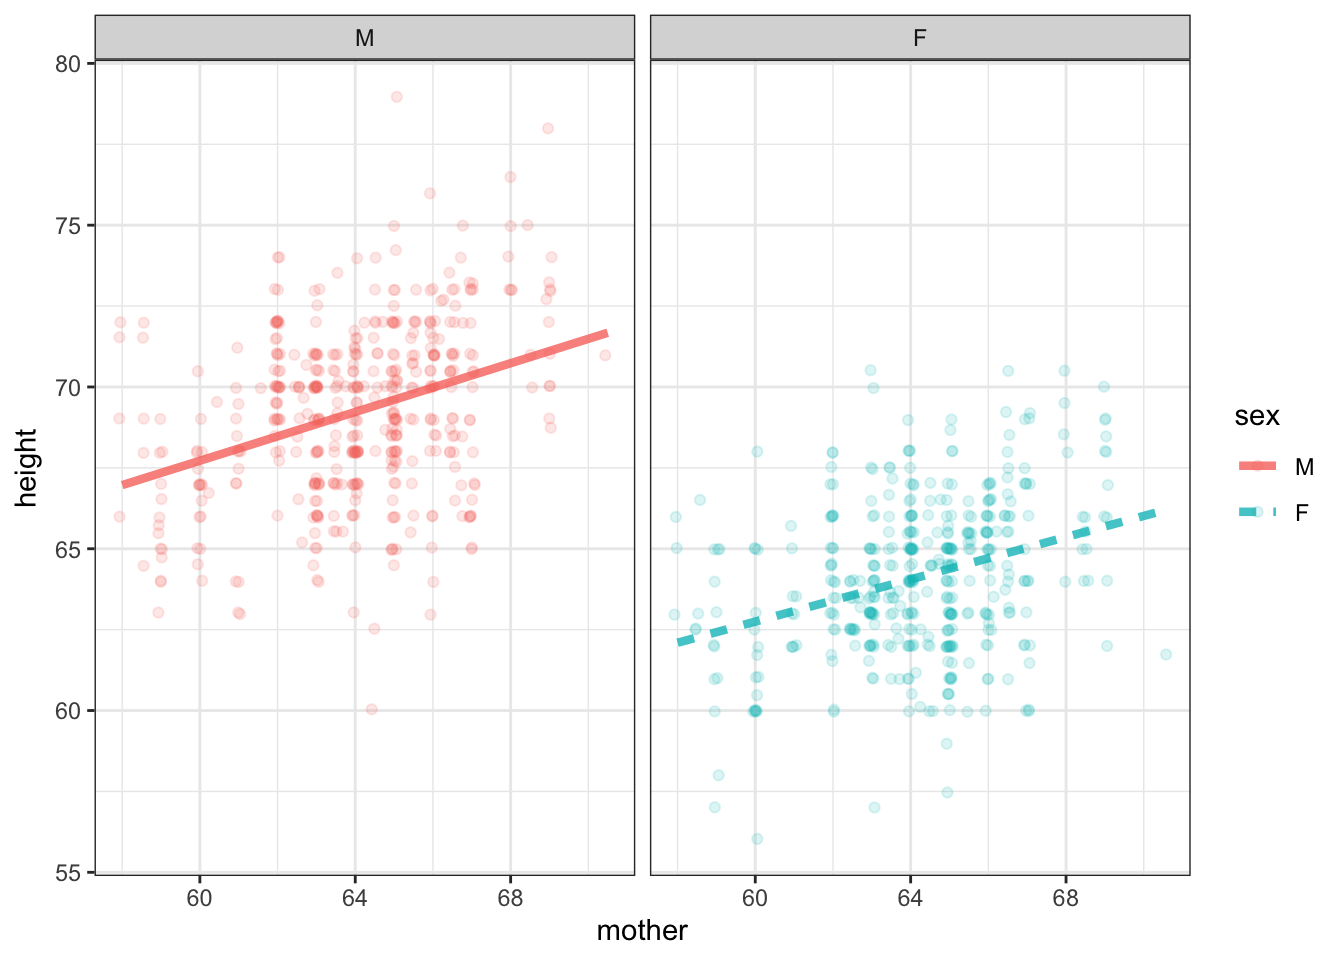
\includegraphics[width=0.8\linewidth]{045-Multiple-explanatory_files/figure-latex/mother-plus-sex-1} \caption[Figure 3: A model of height with two explanatory variables: the mother's height and the child's sex. Each explanatory variable added to a model makes it possible for the model more faithfully to reproduce the response variable.]{Figure 3: A model of height with two explanatory variables: the mother's height and the child's sex. Each explanatory variable added to a model makes it possible for the model more faithfully to reproduce the response variable.}\label{fig:mother-plus-sex}
\end{figure}



\hypertarget{covariates}{%
\section{Covariates}\label{covariates}}

This is a good time to introduce an important concept in statistical modeling. It doesn't have directly to do with the mechanics of statistical inference, but it is critical to interpreting models with multiple explanatory variables.

Often, there is particular interest in the relationship between two variables. Galton's interest was in the relationship between the parents' height and the child's height. There may be other factors involved in the system -- with height a major factor is the sex of the child, but there could be others such as nutrition, health, etc.

Common sense suggests holding these other factors constant so that you can look specifically at the single explanatory variable of particular interest. In the 1880s, Galton did this, for example, by considering only the heights of boys rather than the heights of all children. Within a few years of Galton's work, statisticians had developed techniques to build models with multiple explanatory variables, like Figure 3, which broadened the notion of ``holding other factors constant'' to include accounting for those factors in a model.

The factors that the modeler wants to hold constant are called \emph{covariates}. Really this is just a name for an explanatory variable which is not of direct interest to the modeler, but which the modeler thinks might be playing a role in the system and can't be ignored.

It takes just the most basic notion of biology to realize that when it comes to the relationship between mother's and child's height another potentially important covariate is the height of the father. Figure 4 shows two such models. The model in 4(a) was constructed to have 3 degrees of freedom; 4(b) has 7 degrees of freedom.



\begin{figure}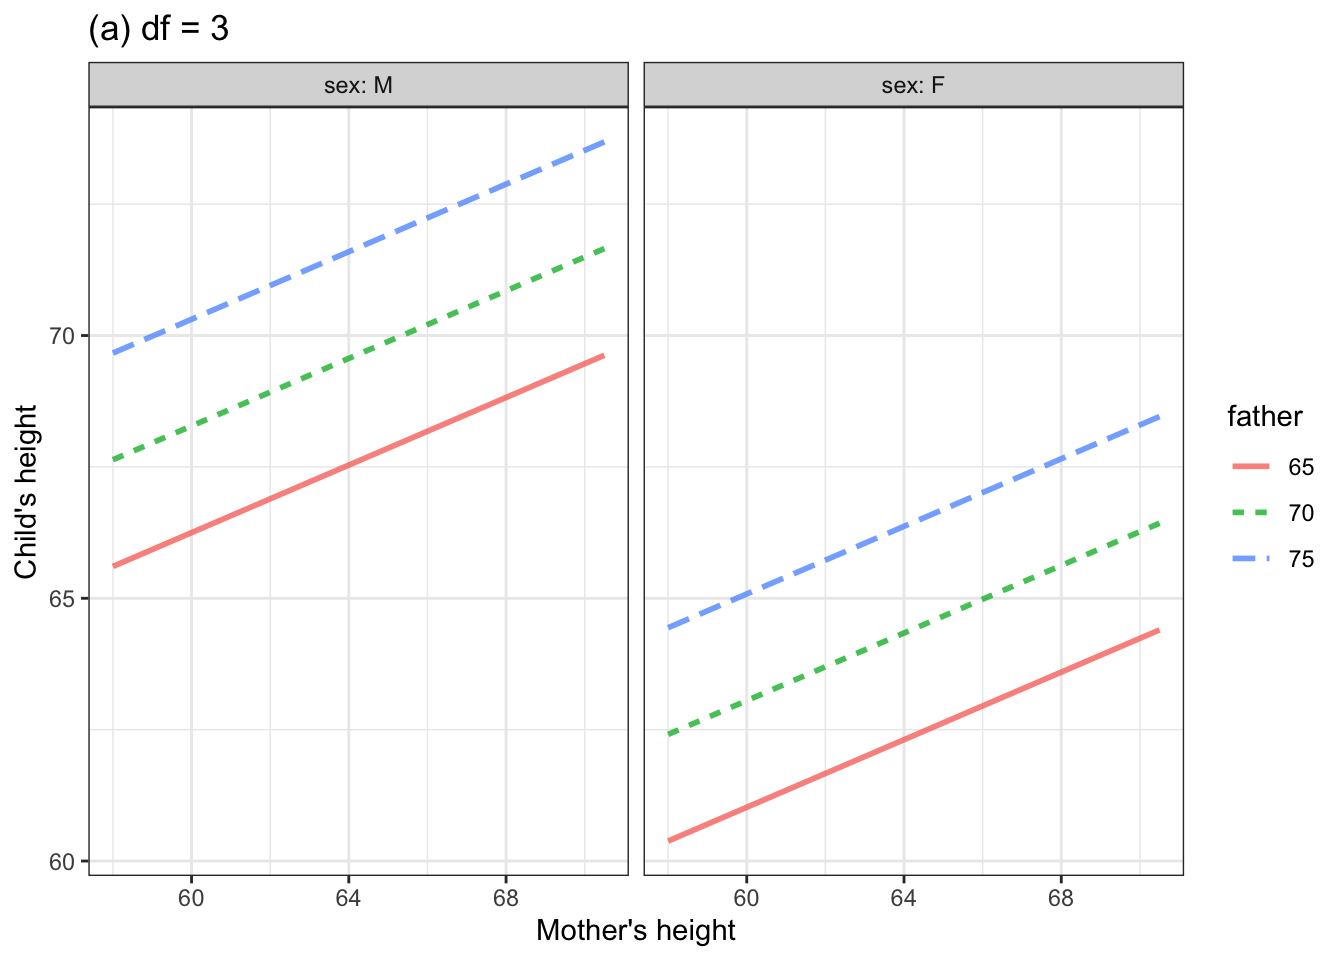
\includegraphics[width=0.8\linewidth]{045-Multiple-explanatory_files/figure-latex/mother-plus-sex-father-1} \caption[Figure 4. Two models of child's height versus mother's height. Father's height and child's sex are included as explanatory variables. Although father's height is a quantitative variable, the graph shows the model for only three, evenly spaced, discrete values.]{Figure 4. Two models of child's height versus mother's height. Father's height and child's sex are included as explanatory variables. Although father's height is a quantitative variable, the graph shows the model for only three, evenly spaced, discrete values.}\label{fig:mother-plus-sex-father}
\end{figure}
\begin{figure}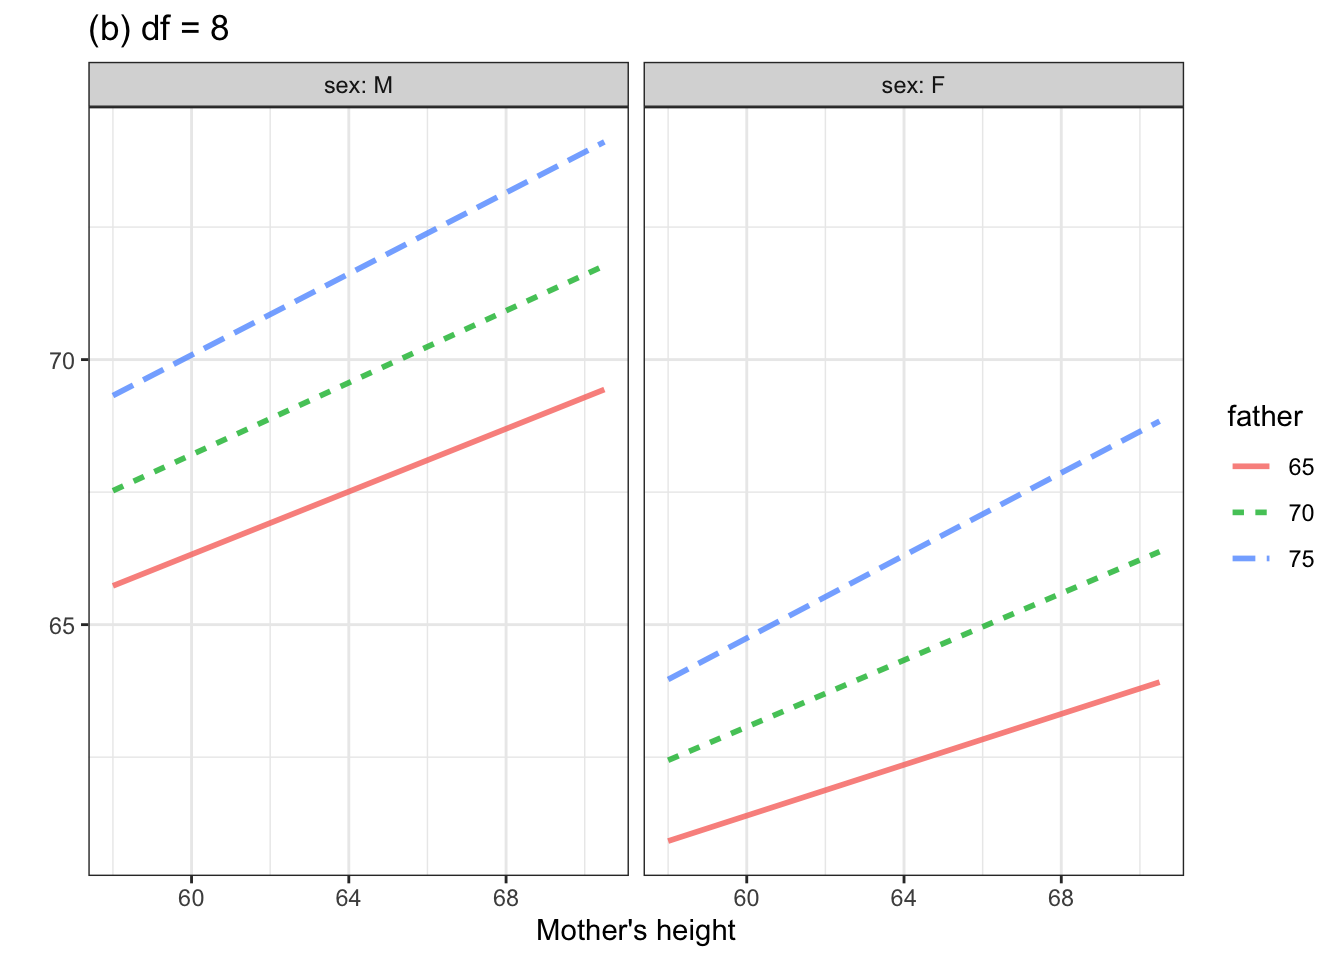
\includegraphics[width=0.8\linewidth]{045-Multiple-explanatory_files/figure-latex/mother-plus-sex-father-2} \caption[Figure 4. Two models of child's height versus mother's height. Father's height and child's sex are included as explanatory variables. Although father's height is a quantitative variable, the graph shows the model for only three, evenly spaced, discrete values.]{Figure 4. Two models of child's height versus mother's height. Father's height and child's sex are included as explanatory variables. Although father's height is a quantitative variable, the graph shows the model for only three, evenly spaced, discrete values.}\label{fig:mother-plus-sex-father}
\end{figure}

Comparing the two models, you might see how a larger df corresponds to increased flexibility.

You might also note from Figure 4 that the model with 8 degrees of freedom suggests that the taller is that father, the more influence the mother has on child's height. The methods of statistical inference let us examine whether this claim is actually justified.

\hypertarget{flexibility-literally}{%
\section{Flexibility, literally}\label{flexibility-literally}}

Chapter 5 imagined a contest between two students, Linus and Curly, for the best model. Let's return to that example, but now we'll construct some models that are more \emph{flexible} than a straight line.




\begin{figure}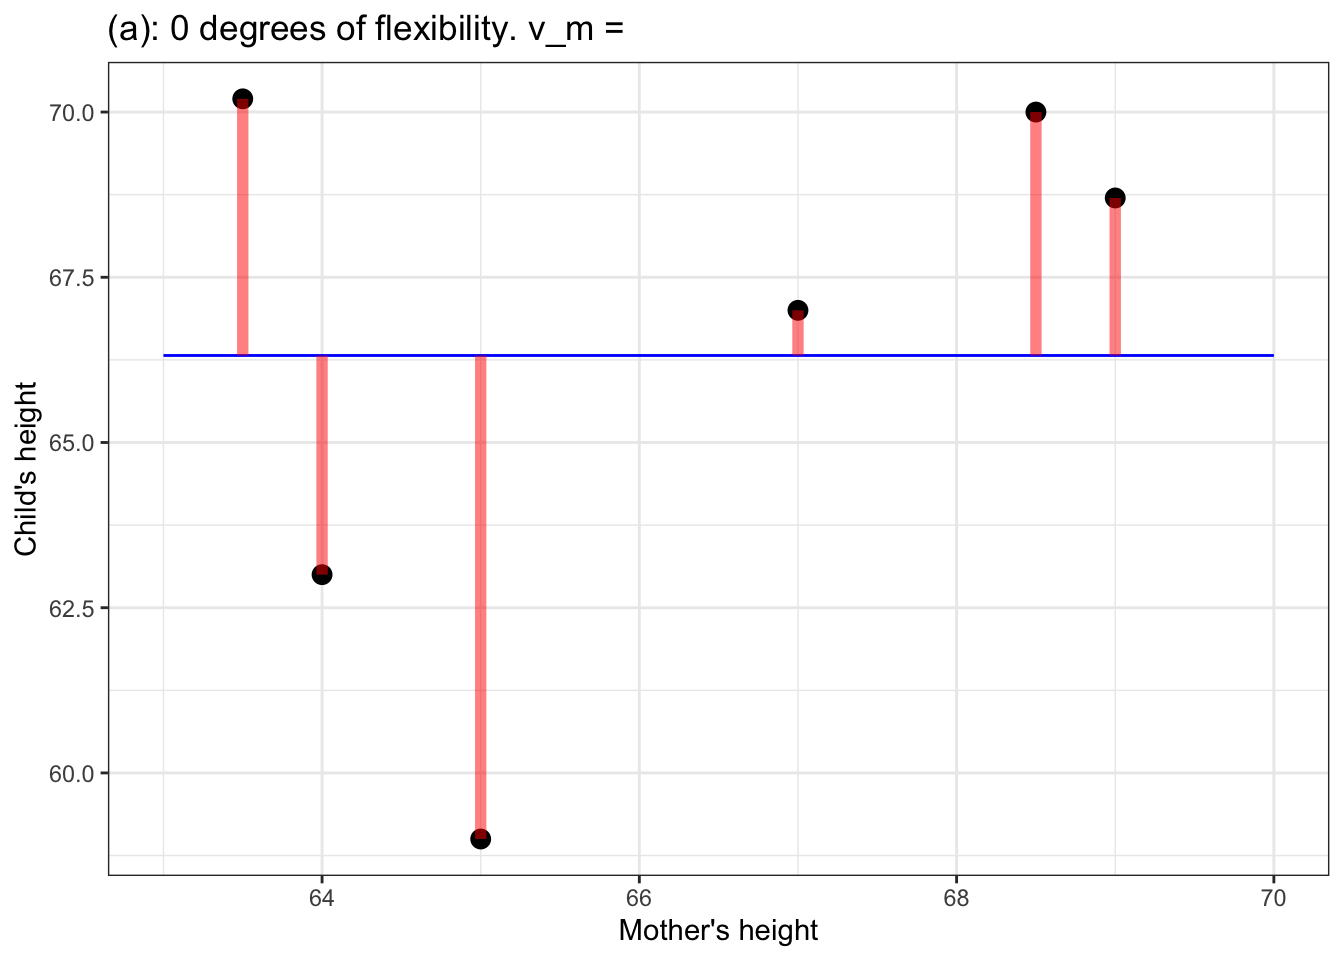
\includegraphics[width=0.5\linewidth]{045-Multiple-explanatory_files/figure-latex/several-df-1} \caption[Figure 5: (a) a flat model -- zero degrees of flexibility; (b) a straight-line model -- one degree of flexibility; (c)
a model with one bend -- two degrees of flexibility; (d) a model with two bends -- three degrees of flexibility."]{Figure 5: (a) a flat model -- zero degrees of flexibility; (b) a straight-line model -- one degree of flexibility; (c)
a model with one bend -- two degrees of flexibility; (d) a model with two bends -- three degrees of flexibility."}\label{fig:several-df}
\end{figure}
\begin{figure}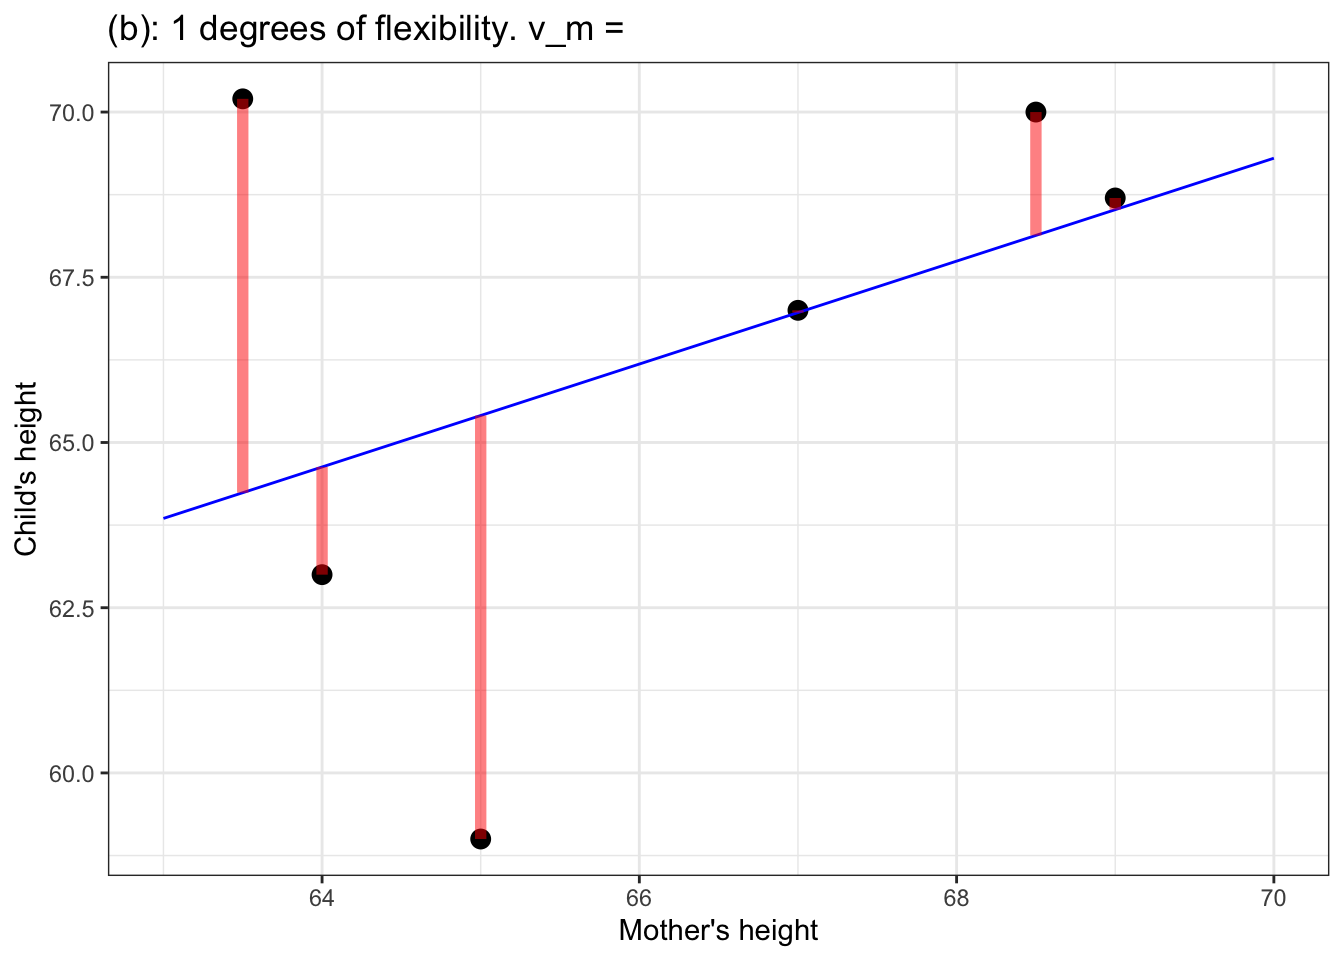
\includegraphics[width=0.5\linewidth]{045-Multiple-explanatory_files/figure-latex/several-df-2} \caption[Figure 5: (a) a flat model -- zero degrees of flexibility; (b) a straight-line model -- one degree of flexibility; (c)
a model with one bend -- two degrees of flexibility; (d) a model with two bends -- three degrees of flexibility."]{Figure 5: (a) a flat model -- zero degrees of flexibility; (b) a straight-line model -- one degree of flexibility; (c)
a model with one bend -- two degrees of flexibility; (d) a model with two bends -- three degrees of flexibility."}\label{fig:several-df}
\end{figure}
\begin{figure}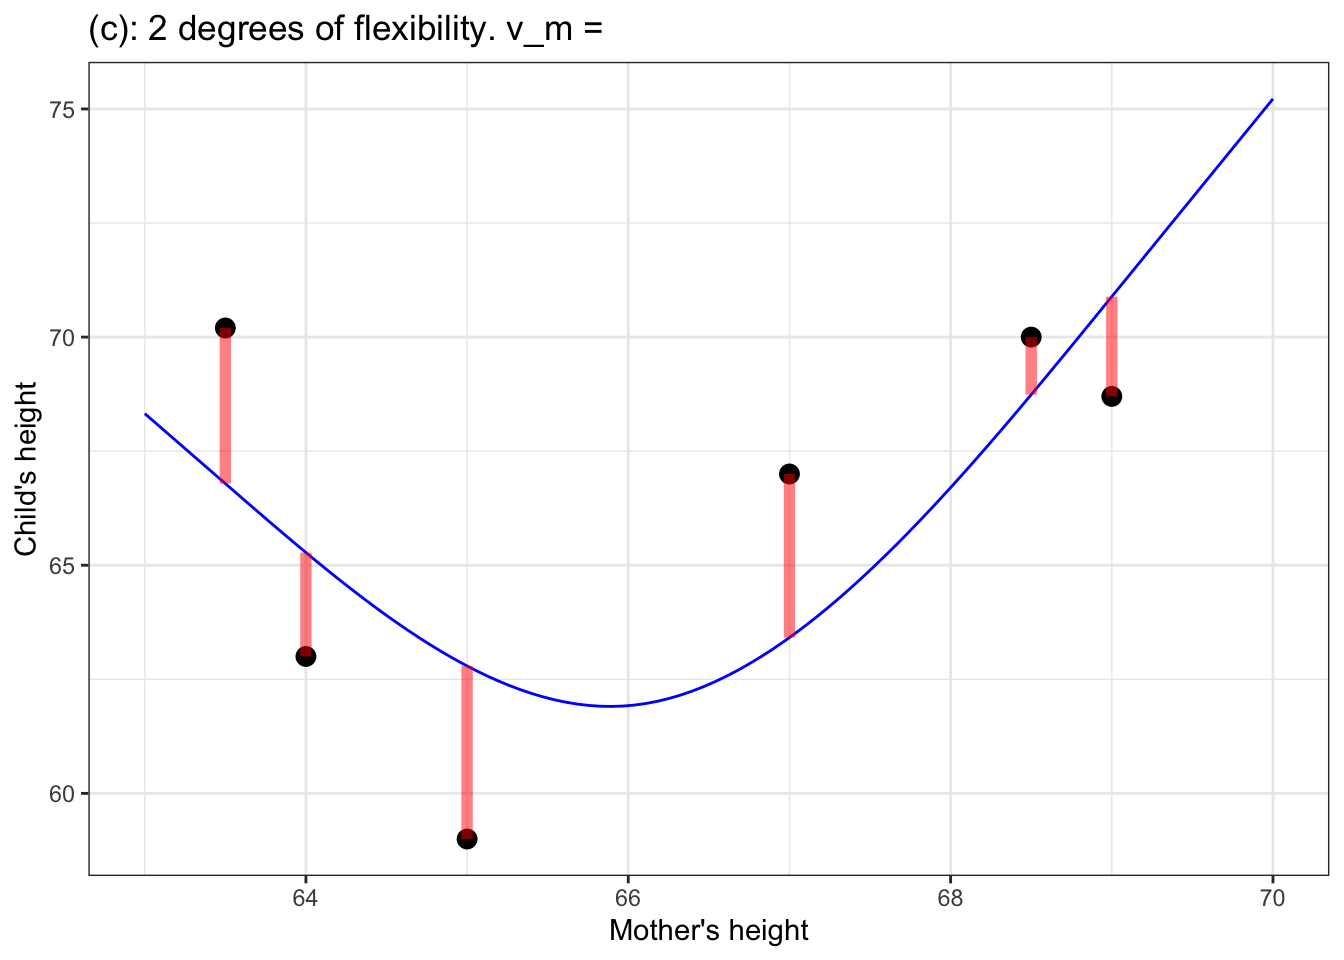
\includegraphics[width=0.5\linewidth]{045-Multiple-explanatory_files/figure-latex/several-df-3} \caption[Figure 5: (a) a flat model -- zero degrees of flexibility; (b) a straight-line model -- one degree of flexibility; (c)
a model with one bend -- two degrees of flexibility; (d) a model with two bends -- three degrees of flexibility."]{Figure 5: (a) a flat model -- zero degrees of flexibility; (b) a straight-line model -- one degree of flexibility; (c)
a model with one bend -- two degrees of flexibility; (d) a model with two bends -- three degrees of flexibility."}\label{fig:several-df}
\end{figure}
\begin{figure}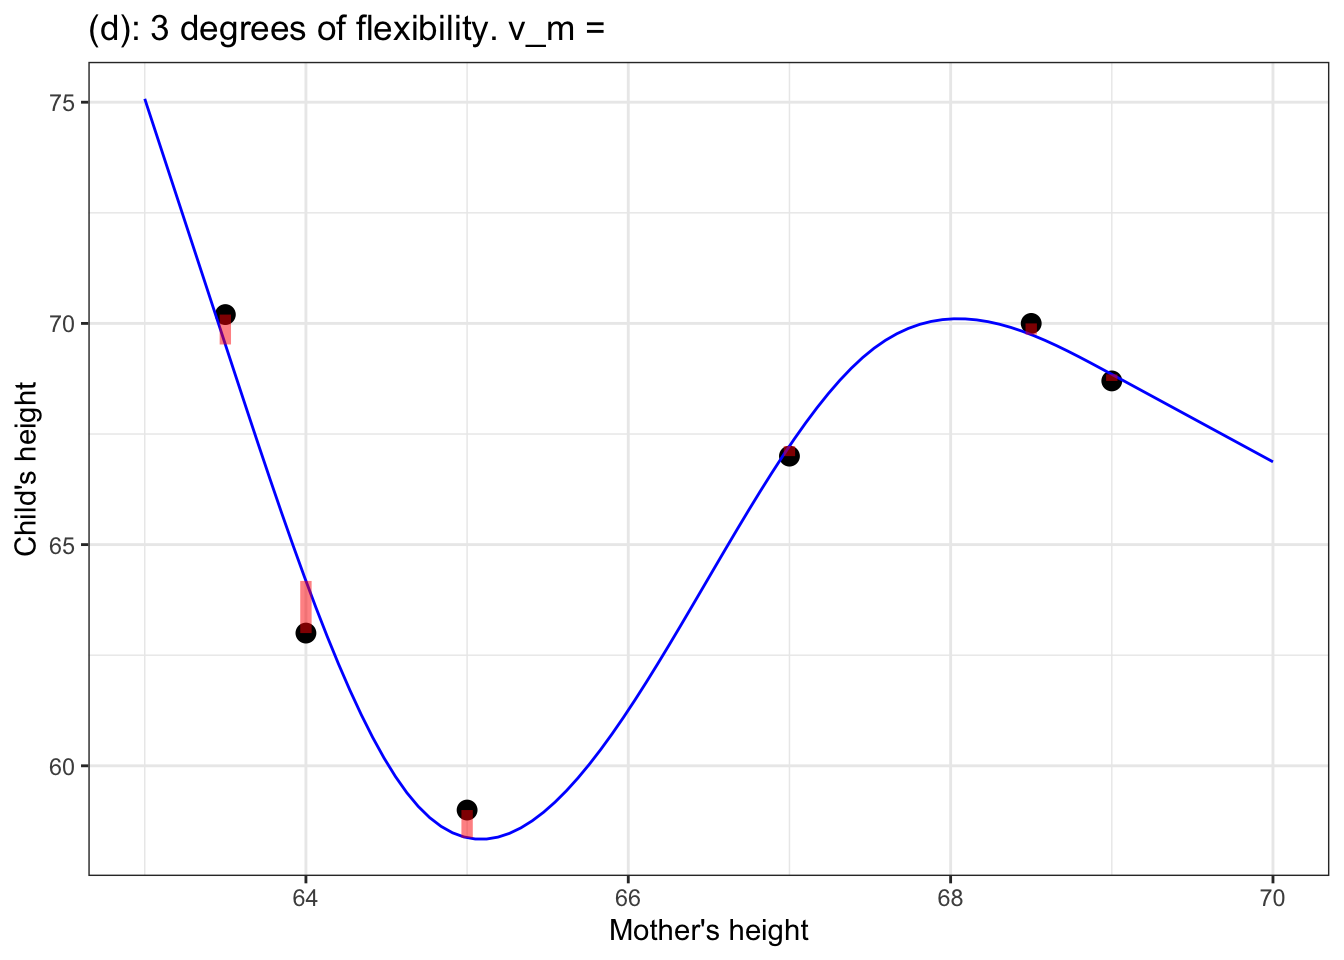
\includegraphics[width=0.5\linewidth]{045-Multiple-explanatory_files/figure-latex/several-df-4} \caption[Figure 5: (a) a flat model -- zero degrees of flexibility; (b) a straight-line model -- one degree of flexibility; (c)
a model with one bend -- two degrees of flexibility; (d) a model with two bends -- three degrees of flexibility."]{Figure 5: (a) a flat model -- zero degrees of flexibility; (b) a straight-line model -- one degree of flexibility; (c)
a model with one bend -- two degrees of flexibility; (d) a model with two bends -- three degrees of flexibility."}\label{fig:several-df}
\end{figure}

In the models in Figure 5, the degrees of flexibility indicate the shape of the function. A flat line has no degrees of flexibility. A sloped line has one degree of flexibility. Adding a bend adds another degree of flexibility, so 3 degrees of flexibility corresponds to two bends.

Notice that as the degree of flexibility goes up, the model function gets closer to the data points. Correspondingly, the variance of the model values, \(v_m\), goes up with increasing degrees of flexibility.

The point of counting degrees of flexibility is to be able to adjust \(v_m\) to take into account the intrinsic nature of flexibility to match more closely the response values. For sufficiently high degrees of flexibility, a model will be able almost perfectly to reproduce the response variable, even when there is \emph{no relationship} between the response and explanatory variables.

\hypertarget{effect-size}{%
\chapter{Effect size}\label{effect-size}}

An \emph{effect size} tells how the output of a model changes when a simple change is made to the input. Many statistical claims are made in terms of an effect size. For instance, according to the \href{https://www.nhtsa.gov/risky-driving/seat-belts}{US National Highway Traffic Safety Administration (NHTSA)}, wearing seat belts reduces the risk of fatal injury to passenger-vehicle occupants by about 50\%. This is an effect size.\footnote{I'm using ``about'' here since we haven't yet introduced confidence intervals. That will happen in Chapter 9. It took some work to chase down the confidence intervals on the relative risk of fatal injury: it is 40\% to 60\%.}

But this related fact from NHTSA is \emph{not} an effect size: 51\% of male passenger-vehicle occupants killed in 2017 were not wearing seat belts.

An effect size summarizes a comparison between two different conditions. In the first example, those two conditions are 1) wearing a seat belt and 2) not wearing a seat belt. In the second example, however, there is just one condition: being a male passenger-vehicle occupant who died in a car accident in 2017.\footnote{What to call a descriptive quantity like 51\%. It's not an effect size. One word used is ``statistic,'' which is simply a number calculated from data. But ``statistic'' has other meanings as well. An effect size is also a statistic. I suggest simply using ``proportion'' for the 51\%. Chapter 11 looks at confidence intervals on means and proportions. The confidence interval for the 51\% proportion is 50-52\%.}

\hypertarget{slopes-and-differences}{%
\section{Slopes and differences}\label{slopes-and-differences}}

Consider two models introduced in Chapter 5. Figure 5.1 shows child's height versus mother's height in Galton's data. The straight-line model shows a slight upward slope. To calculate the effect size of child's height \emph{with respect to} mother's height, pick two values of mother's height: say 60 and 68 inches. From the graph you can read the output of the model at these two values of the input. At an input of 60 inches, the output is 65.5 inches. At an input of 68 inches, the output is (coincidentally) 68 inches. The effect size is the slope of the model: rise over run. Here, the ``run'' is 68 - 60 = 8 inches. The ``rise'' is 68 - 65.5 = 2.5 inches. So the slope is 2.5 / 8 = 0.31.

The model in Figure 5.1 has a quantitative explanatory variable: mother's height. In constrast, the model in Figure 5.2 has a categorical explanatory variable: pollen shape. To calculate an effect size \emph{with respect to pollen shape} in Figure 5.2, follow much the same procedure. First, pick the two input levels you want to compare. Here, there are only two levels possible: long and round shapes. Next, look up the model output at each of the two inputs. The output of the model is framed as a probability. The probability of a white flower is 24\% for long pollen, and 25\% for round pollen.

Since the explanatory variable is categorical, it doesn't mean much to look at the numerical difference in the input. The model output, on the other hand, is quantitative (as it is for all the models we consider in this book). The effect size is 25\% - 24\% = 1 percentage point.

To recap, when the explanatory variable is \emph{quantitative}, the effect size is stated as a \emph{slope}: change in output divided by change in input. When the explanatory variable is \emph{categorical}, the effect size can be stated as a \emph{difference}.

\hypertarget{risk}{%
\section{Risk}\label{risk}}

In the previous paragraph, I say ``\emph{can} be stated as a difference'' because there are other ways often used to compare the model output between two different levels of a categorical explanatory variable. For instance, when the output is interpreted as a ``risk,'' the two outputs might be compared as a \emph{ratio}, called the \emph{risk ratio}. It sounds odd when talking about flower color, but if we were thinking about the ``risk'' that a pea plant's flowers are white, then it would be appropriate to consider the effect size with respect to pollen shape as the ratio 25\% / 24\% = 1.04. Note that this 1.04 is not in percent. When writing about risk ratios, people often use percentage terms. The risk ratio of 1.04 might be described, ``The risk of a white flower increases by 4 percent.'' Were the risk ratio smaller than 1, say 0.87, we would speak of a risk \emph{decrease}: ``The risk of a white flower is 13\% lower for \ldots{}.''

It's potentially confusing for us to report \emph{differences} of risk in ``percentage points'' and \emph{ratios} of risk as ``percent.'' Not everyone is sensitive to the distinction between ``percentage points'' and ``percent.'' Perhaps it would be helpful to report differences as an \emph{absolute} change in risk while ratios are a \emph{relative} change in risk.

There's yet another way used to describe changes in risk: the \emph{odds ratio}. Odds are a different format for describing risk. If the probability of an outcome is \(p\), the odds are \(p/(1-p)\). So, the odds of a white flower in a plant which has round pollen is \(0.25/(1-0.25) = 0.25 / 0.75 = 1/3\). The use of odds, and its cousin, \emph{log odds}, is a genuine help when working with models with multiple explanatory variables.

\hypertarget{simple-changes-in-input}{%
\section{Simple changes in input}\label{simple-changes-in-input}}

I'm using the word ``simple'' to refer to the change in input involved in an effect size. Several considerations motivate this:

\begin{itemize}
\tightlist
\item
  When looking at a categorical explanatory variable, and effect size is a comparison of just two of the levels.
\item
  When looking at a quantitative explanatory variable, I advocate using a \emph{finite} change in input, e.g.~the 60 inches to 68 inches in mother's height. That's simpler than the alternative, using an \emph{infinitesimal} change in input, and more appropriate for many machine-learning models where the output can vary discontinuously as the input changes.
\end{itemize}

But the main thing I want to emphasize with the word ``simple'' has to do with models with multiple explanatory variables. In such models, there are different effect sizes for the different explanatory variables. That is, an effect size reports the change in model output when a \emph{single} explanatory variable is changed, holding all the others constant. This is where the phrase ``with respect to'' comes into play. For instance, the model displayed in Figure 4 of Chapter 6, with child's height as the response variable, involves three explanatory variables: mother's height, father's height, and child's sex. An effect size in such a model refers to a specific explanatory variable. So it's meaningful to speak of the effect (on child's height) with respect to mother's height, or the effect with respect to father's height, or the effect with respect to child's sex. Which one is right for you depends on what you are investigating.

\hypertarget{f-and-r}{%
\chapter{F and R}\label{f-and-r}}

We now have the pieces we need to assemble the central quantity which informs statistical inference. These are:

\begin{enumerate}
\def\labelenumi{\arabic{enumi}.}
\tightlist
\item
  \(n\), the sample size (or, more concretely, the number of rows in out data frame)
\item
  \(v_r\), the variance of the response variable. \(v_r\) for binary categorical response variables is based on the 0-1 encoding.
\item
  \(v_m\), the variance of the model values.
\item
  \(df\), the \emph{degree of flexibility}.\footnote{This is a non-standard name. The convention is to refer to the quantity \(n - (df + 1)\) as the \emph{degrees of \textbf{freedom}}.}
\end{enumerate}

We'll put these together to form a quantity called F. (The name, F, is in honor of Ronald Fisher, one of the leading statisticians of the first half of the 20th.) The formula for F is pretty simple, so I'll present it right here for ready reference.

\[F \equiv \frac{n - (1 + df)}{df} \frac{v_m}{v_r - v_m}\]
For almost all the settings considered in introductory statistics courses, \(df\) is 1, so the formula simplifies to:
\[F =  (n-1) \frac{v_m}{v_r - v_m}\]

\hypertarget{whats-the-meaning-of-f}{%
\section{What's the meaning of F?}\label{whats-the-meaning-of-f}}

F combines the four quantities \(n\), \(v_r\), \(v_m\), and \(df\). To get a notion why the combination works, keep these basic ideas in mind concerning what it means to have ``more evidence.''

\begin{itemize}
\tightlist
\item
  The larger \(n\), the more evidence. That's why F is more-or-less proportional to \(n\). (Strictly speaking, F is proportional to \(n - (1+df)\).)
\item
  The more complicated the model -- e.g.~the number of explanatory variables or levels in an explanatory categorical variable -- the less evidence. Or, put another way, we would want more evidence from data to justify a complicated model than a simple model. The division by \(df\) in the formula for F implements this idea.
\item
  The closer the model values come to capturing the actual response variable, the greater the evidence that there is a relationship. An obvious
  way to quantify this closeness are with the difference \(v_r - v_m\). We want the size of F to increase as \(v_m\) gets closer to \(v_r\). So F is proportional to \(\frac{1}{v_r - v_m}\).
\item
  But the numerical value of the difference \(v_r - v_m\) depends on the units in which the response variable is measured. For instance, we could express the running times in Chapter 1 in minutes or in seconds. But the difference \(v_r - v_m\) would be \(60^2 = 3600\) times larger if we used seconds than minutes. Obviously we don't want our F value to depend on the units used. To avoid that, we divide \(v_r - v_m\) by \(v_m\), getting the \(v_m / (v_r - v_m)\) in the formula for F.
\end{itemize}

\hypertarget{r-squared}{%
\section{R-squared}\label{r-squared}}

Many people prefer to look at a ratio \(v_m / v_r\) to quantify how close the model values are to the values of the response variable. If the model does a good job accounting for the response variable, then \(v_m\) will be close to \(v_r\). That is, the ratio will be close to 1. On the other hand, if the model tells us little or nothing about the response variable, \(v_m\) will be close to zero and the ratio itself will be zero.

The ratio has a famous name: *R-squared\$, that is:

\[R^2 = v_m / v_r\]
Another, more obscure name for \(R^2\) is \emph{coefficient of determination}, which is awkward but does express the point that \(R^2\) is about the extent to which the explanatory variables, when passed through the model, determine the response variable.

\begin{itemize}
\tightlist
\item
  Biggest possible \(R^2\) is 1, which can only occur when the model values are exactly the same as the values of the response variable.
\end{itemize}

\(R^2\) is, literally, the faction of the variation in the response variable that has been captured by the model.

\begin{itemize}
\tightlist
\item
  \(R^2\) is never negative. This is part of the reason why keeping track of \(df\) is important when there are multiple explanatory variables, or, to be more precise, multiple explanatory vectors.
\end{itemize}

\hypertarget{f-in-statistics-books}{%
\section{F in statistics books}\label{f-in-statistics-books}}

In most statistics book, F is not written in the form above but in one of a couple of alternative -- but equivalent -- forms. There's no particular reason to use these forms. Knowing what they look like will help you make sense of traditional statistical reports.

Since \(R^2\) summarizes the relationship between \(v_m\) and \(v_r\), the formula for F can be written in terms of \(R^2\). This is the first of the alternative forms.

\[F = \frac{n - (1+df)}{df} \frac{R^2}{1 - R^2}\]

Another alternative form comes from using an intermediate in the calculation of \(v_m\) and \(v_r\). Recall how the variance is calculated by calculating square differences and averaging. To average, of course, you add together the quantities and then divide by the number of quantities being averaged.

Suppose you didn't bother to average, and stopped after adding up the square differences. The name for this intermediate is the \emph{sum of squares}.
F is often written in terms of the sum of squares of the response variable SS\_r\_ and of the model values SS\_m\_. Something like this:

\[F = \frac{n - (1+df)}{df} \frac{\mbox{SS}_m}{\mbox{SS}_r - \mbox{SS}_m}\]

More typically, instead instead of looking at the model values directly, the tradition in classical inference is to consider what's called the \emph{sum of squares of the residuals}, which is simply SSR = \(\mbox{SS}_r - \mbox{SS}_m\) and the formula is re-written like this:

\[F = \frac{\mbox{SS}_m / df}{SSR / (n -  (1+df))}.\]
Both the numerator and the denominator of this ratio have the form of a sum of squares divided by a count. In the terminology of classical inference, such things are called \emph{mean squares}.

In this book, we'll just use the formula for F given at the start of this chapter. The others give exactly the same value, but let's avoid having ton work with potentially confusing vocabulary such as the mean square and sum of squares.

\hypertarget{confidence-intervals}{%
\chapter{Confidence intervals}\label{confidence-intervals}}

We use effect size to quantify how a change in an explanatory input changes the output of the statistical model.

Example:

One way to express our uncertainty due to limited data in the effect size is to state it as an \emph{interval} rather than a single number. Classical inference developed several ways of finding an appropriate interval. This is called a confidence interval.

\hypertarget{confidence-intervals-from-f}{%
\section{Confidence intervals from F}\label{confidence-intervals-from-f}}

In the case of the simplest models, where \(df = 1\), the interval can be calculated directly from F and the effect size B. The formula is

\(CI = B (1 \pm \sqrt{4/F}).\)

Example:

\hypertarget{why-4}{%
\section{Why 4?}\label{why-4}}

\hypertarget{situations-where-f-doesnt-tell-enough}{%
\section{Situations where F doesn't tell enough}\label{situations-where-f-doesnt-tell-enough}}

When there are multiple effect sizes from different variables.

Still, the F formula works pretty well so long as the different explanatory vectors are independent of one another (orthogonal). {[}DOES IT{]}

\hypertarget{so-called-statistical-significance}{%
\chapter{So-called ``statistical significance''}\label{so-called-statistical-significance}}

In this book we've used effect size as the basic measure of how a response variable is related to an explanatory variable. The confidence interval of an effect size tells what range of values are consistent with our data. When that interval includes zero, it's fair to say that our data do not rule out the possibility that there is no effect at all, that is, that the response and explanatory variables are unrelated.

For historical reasons, its common for researchers to present their results as ``statistically significant.'' The way a relationship between a respose and explanatory variable(s) can win the certificate of ``statistical significance,'' is by a process called \emph{null hypothesis testing}. A null hypothesis test involves calculating a quantity known as the p-value, which is always between 0 and 1. When the p-value is smaller than 0.05 (by convention), the researcher is warranted in using the label ``statistically significant.''

First, I'll handle the question of how the calculation is done. Then, I'll give some history and recent professional recommendations that the result of the calculation has no meaning. Hopefully, despite the ubiquity of p-values in conventional statistics textbooks and in the research literature, you'll be able to use more meaningful ways to describe the relationship, if any, between response and explanatory variables.

\hypertarget{calculating-a-p-value}{%
\section{Calculating a p-value}\label{calculating-a-p-value}}

When you quantify the relationship between a response and explanatory variable(s), several inferential quantities are generated. In this book, we focus particularly on F and the degrees of flexibility \(df\), from which everything else flows.

The p-value calculation takes F, \(df\) and sample size \(n\) as inputs and produces an output in the form of a probability, that is, a number between 0 and 1. The calculation from first principles is very difficult, so everyone builds on the earlier work of couragious statisticians and mathematicians who have simplifed it into looking up a number in a table, or, more conveniently, asking a computer to look up the number.

For example, in the R computing language, the function \(pf()\) does the calculation. Specifically, the p-value is \texttt{1\ -\ pf(F,\ df,\ n\ -\ \ df)}. In many software systems, such as Excel, all of the F, \(df\) and p-value calculations are packaged together in functions that are often called ``tests.'' There are often many such ``tests'' provided for different settings like the difference between two means or the slope of a regression line. But the underlying principles are those presented here in a unified way, with \(v_r\), \(v_m\), \(df\), and F.

Since what you do with a p-value is to compare it to 0.05, there is a remarkably simple way to go. instead of making the rule about the size of the p-value, we make it about the size of F. The value of F that corresponds to \(p = 0.05\) is called the ``95\% critical value'' of F. This is often written F\(^\star\). So long as you have \(n\) moderately large, say \(n \gtrapprox 10\), the critical value is 4. That's it. 4. If \(n \gtrapprox 10\), F=4 is the threshold for declaring a relationship ``statistically significant.''

For \(n\) small, it's no longer adequate to use 4 as the critical value. Instead, for all the situations encountered in an introductory statistics class, you have to look up the critical value in Figure 1.

\begin{longtable}[]{@{}llllllllll@{}}
\toprule
Sample size \(n\) & large & 10 & 9 & 8 & 7 & 6 & 5 & 4 & 3\tabularnewline
\midrule
\endhead
F\(^\star\) & 4 & 5 & 5.3 & 5.6 & 6 & 7 & 8 & 10 & 19\tabularnewline
\bottomrule
\end{longtable}

**Figure 1: Critical values for F depend on the sample size \(n\), especially for small \(n\). These critical values are for \(df=1\).

Do remember that the formula for F includes \(n\). One way to get a large F is to use data with large \(n\). So don't mis-interpret the table as saying \sout{``10 points is enough.''} It's just that F\(^\star\) doesn't much depend on \(n\) when \(n \gtrapprox 10\).

Figure 1 is for \(df = 1\), which is the situation in most of the settings used in introductory statistics. For larger \(df\), the critical values of F are similar except for models where \(df \approx n\). See Figure 3, below.

\hypertarget{history-and-criticism}{%
\section{History and criticism}\label{history-and-criticism}}

In the 1880s a way of quantifying the relationship between two numerical variables was invented. It was called the \emph{correlation coefficient} and it continues to be used to this day. Probably it should not be so widely used today as it is, because we now have effect sizes to work with and because of the challenges to interpreting the correlation coefficient, as you'll see.

The correlation coefficient from the 1880s is closely related to the \(R^2\) statistic introduced in Chapter 6. Specifically, the size of the correlation coefficient is \(r = \sqrt{R^2} = R\). Recall that \(R^2\) is the ratio of the variance of model values to the variance of the response variable:

\[R^2 \equiv v_m / v_r.\]

Recall as well that each of \(v_m\) and \(v_r\) are an average of square differences, and, of course, a square of a real number cannot be less than zero. Consequently, \(R^2\) cannot be negative.

If \(R^2\) is exactly zero, it's reasonable to conclude that the explanatory variable(s) cannot account for the response variable. Seen another way, if \(R^2\) is zero then \(v_m\) must also be zero. For \(v_m\) to be zero, all of the model values must be exactly the same, so the effect size must also be zero.

What happens if -- to do a thought experiment -- the response variable is completely unrelated to the explanatory variable? You might be anticipating that \(R^2\) will be zero. In practice, however, it's not. This comes about because there are almost always associations happening purely at random that, when quantified, produce \(R^2 > 0\). So, in deciding whether the data indicate a relationship between the response and explanatory variable(s), we need to decide what value of \(R^2\) is so close to zero as to be a sign that the response and explanatory variable(s) are related.

This question was asked, and answered, early in the 1900s. In one specific case, it was asked by a man named Dr Shaw at the January 15, 1907 meeting of the Royal Statistical Society in the UK. The context was a discussion of a paper by \href{https://en.wikipedia.org/wiki/Reginald_Hawthorn_Hooker}{Reginald Hooker} who had studied the correlation between weather and crops. In Table 1 of his paper, part of which is reproduced in Figure 1, Hooker presented the correlation between amount of wheat harvested and the amount of rain accumulated over the previous seasons. He also looked at the correlation of wheat harvest and temperature -- that's the second numerical column in Figure 2.

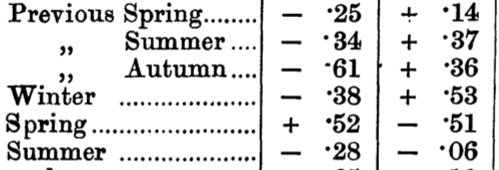
\includegraphics[width=0.8\linewidth]{images/Hooker-correlations}

Now to quote from the recollections published in 1908 by \href{https://en.wikipedia.org/wiki/William_Sealy_Gosset}{William Seely Gossett}, writing anonymously as ``Student'':

\begin{quote}
\emph{Dr Shaw made an enquiry as to the significance of correlation coefficients derived fronm small numbers of cases.}
\end{quote}

The small number here is 21: Hooker had worked with 21 years of crop and weather data. The plain meaning of ``significance of'' here is ``the meaning carried by.'' A modern person might have asked, ``Some of those correlations are pretty small. And you don't have much data. Do such small correlations mean anything?'' To continue \ldots{}

\begin{quote}
\emph{His question was answered by Messrs \href{https://en.wikipedia.org/wiki/Udny_Yule}{Yule} and \href{https://en.wikipedia.org/wiki/Reginald_Hawthorn_Hooker}{Hooker} and Professor \href{https://en.wikipedia.org/wiki/Francis_Ysidro_Edgeworth}{Edgeworth}, all of whom considered that Mr Hooker was probably safe in taking .50 as his limit of significance for a sarnple of 21.}
\end{quote}

In plainer language: don't take as meaningful any correlation coefficient less than 0.50.

\begin{quote}
\emph{They did not, however, answer Dr Shaw's question in any more general way. Now Mr Hooker is not the only statistician who is forced to work with very small samples, and until Dr Shaw's question has been properly answered the results of such investigations lack the criterion which would enable us to make full use of them. The present paper, which is an account of some sampling experimiients, has two objects: (1) to throw some light by empirical methods on the problem itself, (2) to endeavour to interest mathematicians who have both time and ability to solve it.}
\end{quote}

A general solution was found, in part by Student but also by others such as Ronald Fisher. Key to setting up the solution was to define ``significance'' in mathematical terms. The setup was logically ingenious and a little hard to follow. It goes like this:

Suppose we have two variables that have been generated entirely at random and independently of one another. We can calculate the correlation coefficient between them. The correlation coefficient will also be a random number, presumably near zero. If we perform the experiment many times and collect the set of random correlation coefficients produced, we will have an idea of what is the size of commonly encountered coefficients, and how big a correlation coefficient should be so that we can sensibly regard it as being unlikely to arise from random, independent variables.

Doing the random-and-independent-variable simulation for the \(n = 21\) situation of Hooker's paper, indicates that a correlation coefficient at or above 0.50 will result about 1\% of the time. That's a small probability. So, as Messrs Yule, Hooker, and Edgeworth said, it seems ``pretty safe'' -- 99\%? -- to conclude that \(r = 0.50\) with \(n=21\) means that there \emph{is} an association between the two variables.

Actually, the simulation only tells us about a hypothetical world -- called the \emph{Null Hypothesis} -- in which variables are random and independent. The simulation doesn't have anything to say about a world in which variables are related to one another. It's legitimate to say that observing something that's very unlikely -- 1\% chance of \(r \ge 0.5\) -- suggests that the data didn't come from that world. But suppose data came from another hypothetical world -- called the \emph{Alternative Hypothesis} -- where variables are related to one another. Such a world might easily generate a value \(r < 0.5\). So seeing large r entitles us to ``reject the null hypothesis,'' but seeing small r doesn't tell us about the alternative hypothesis. Small r just means that we can't reject the null hypothesis. The formal language is ``fail to reject the null hypothesis.''

The probability that comes from the null hypothesis simulation has a name: the \emph{p-value}.

In 1925, Ronald Fisher suggested using a probability of 5\% instead of 1\% in lab work. This guideline was intended to help lab workers avoid making unwarranted claims that an experiment is showing a positive result. If the p-value is \(p > 0.05\), you have nothing to say about your experiment, you \emph{fail to} reject the null hypothesis.

Over the years, this got turned around. When \(p < 0.05\) (by convention), you're entitled to ``reject the null hypothesis.'' In order to publish a scientific report, researchers were obliged to have enough data to reject the null. This is a way of saying that \emph{some} non-null claim is warranted. But which ones? Certainly the point is to show that there is some substantial relationship between the response and explanatory variable(s), a relationship that means something in the real world. Rejecting the null is not, on its own, a sign that the relationship is substantial and meaningful.

Further confusing things was that little word used by Dr Shaw in 1907: \emph{significance}. An equivalence developed between ``reject the null'' and ``significance.'' Claims that had a low p-value came to be described as ``statistically significant.'' In everyday speech, ``significant'' means substantial or meaningful or important. This is \emph{not} the meaning of ``statistically significant.'' The importance or meaning of an association between a response and explanatory variables can be assessed by looking at the \emph{effect size}, and checking whether the effect size is large enough to have practical meaning in the world. But even tiny effect sizes, without any practical implications, can generate small p-values. You just have to have enough data. With the phrase ``statistically significant'' attached to findings, people could publish their work even if there was no practical meaning.

It's worse than this. Even when variables are unrelated, the p-value will be smaller than 0.05 on five percent of occasions. When Fisher was writing in 1925, there weren't many researchers and each lab experiment required a lot of work. And, in any event, ``rejecting the null'' was just an internal check on what lab work is worth following up and replicating. But today there are millions of researchers. And each researcher can easily look at dozens of variables. So, even if every researcher was working with unrelated variables, statistical significance will be found millions of times: enough to saturate the literature and effectively hide genuine findings with practical significance.

After decades of researchers mis-using p-values, in 2019 the American Statistical Association, a leading professional organization world-wide, issued a statement worth quoting in length:

\begin{quote}
\emph{It is time to stop using the term 'statistically significant" entirely. Nor should variants such as ``significantly different,'' ``p \textless{} 0.05,'' and ``nonsignificant'' survive, whether expressed in words, by asterisks in a table, or in some other way.}

\emph{Regardless of whether it was ever useful, a declaration of ``statistical significance'' has today become meaningless. Made broadly known by Fisher's use of the phrase (1925), Edgeworth's (1885) original intention for statistical significance was simply as a tool to indicate when a result warrants further scrutiny. But that idea has been irretrievably lost. Statistical significance was never meant to imply scientific importance, and the confusion of the two was decried soon after its widespread use (Boring 1919). Yet a full century later the confusion persists.}

\emph{And so the tool has become the tyrant. The problem is not simply use of the word ``significant,'' although the statistical and ordinary language meanings of the word are indeed now hopelessly confused (Ghose 2013); the term should be avoided for that reason alone. The problem is a larger one, however: using bright-line rules for justifying scientific claims or conclusions can lead to erroneous beliefs and poor decision making (ASA statement, Principle 3). A label of statistical significance adds nothing to what is already conveyed by the value of p; in fact, this dichotomization of p-values makes matters worse.}

\emph{For example, no p-value can reveal the plausibility, presence, truth, or importance of an association or effect. Therefore, a label of statistical significance does not mean or imply that an association or effect is highly probable, real, true, or important. Nor does a label of statistical nonsignificance lead to the association or effect being improbable, absent, false, or unimportant. Yet the dichotomization into ``significant'' and ``not significant'' is taken as an imprimatur of authority on these characteristics. In a world without bright lines, on the other hand, it becomes untenable to assert dramatic differences in interpretation from inconsequential differences in estimates. As Gelman and Stern (2006) famously observed, the difference between ``significant'' and ``not significant'' is not itself statistically significant.}

\emph{Furthermore, this false split into ``worthy'' and ``unworthy'' results leads to the selective reporting and publishing of results based on their statistical significance---the so-called ``file drawer problem'' (Rosenthal 1979). And the dichotomized reporting problem extends beyond just publication, notes Amrhein, Trafimow, and Greenland (2019): when authors use p-value thresholds to select which findings to discuss in their papers, ``their conclusions and what is reported in subsequent news and reviews will be biased\ldots{}Such selective attention based on study outcomes will therefore not only distort the literature but will slant published descriptions of study results---biasing the summary descriptions reported to practicing professionals and the general public.'' For the integrity of scientific publishing and research dissemination, therefore, whether a p-value passes any arbitrary threshold should not be considered at all when deciding which results to present or highlight.}
\end{quote}

\hypertarget{appendix-when-df-geq-2}{%
\section{\texorpdfstring{Appendix: When \(df \geq 2\)}{Appendix: When df \textbackslash{}geq 2}}\label{appendix-when-df-geq-2}}

For models with multiple explanatory variables or categorical variables with more than two levels, the critical values of F differ substantially from the \(df = 1\) case only for very small \(n\).

\begin{longtable}[]{@{}llllllllll@{}}
\toprule
Sample size \(n\) & large & 10 & 9 & 8 & 7 & 6 & 5 & 4 & 3\tabularnewline
\midrule
\endhead
\(df = 1\) & 4 & 5 & 5.3 & 5.6 & 6 & 7 & 8 & 10 & 19\tabularnewline
\(df = 2\) & 3 & 4.5 & 4.7 & 5.1 & 5.7 & 7 & 9.5 & 19 & 200\tabularnewline
\(df = 3\) & 2.7 & 4.3 & 4.8 & 5.4 & 6.6 & 9.3 & 19 & 216 & NA\tabularnewline
\(df = 4\) & 2.5 & 4.5 & 5.2 & 6.4 & 9.1 & 19 & 225 & NA & NA\tabularnewline
\bottomrule
\end{longtable}

\emph{Figure 3: Critical values for F for small \(n\) and a few different values of \(df\).}

\hypertarget{simple-means-and-proportions}{%
\chapter{Simple means and proportions}\label{simple-means-and-proportions}}

The presentation of classical inferene in this compact guide does not follow the historical flow of how inferential concepts were developed, largely over the half century from 1880 to 1925. Instead we started with F, which dates from 1925, introducing it in the context of models, an even more recent concept. Models provide a means to address contemporary uses of data.

Historically, inference started with very simple questions involving a single variable. For instance, after observing a mental-health patient's sleep over several days, a reasonable presentation of how much sleep the patient got is the the mean over those days. Or, in a more contemporary context, imagine being interested in the trend toward self-driving cars. A reasonable summary of the deployment of the technology could be the proportion of cars on the road with self-driving features such as lane-keeping or automatic braking before a collision.

Very often, behind the interest in a mean or proportion is a different interest: a change in mean or a change in proportion. For such questions, models and F are the way to go. But in this chapter we'll journey into neans and proportions themselves.

\hypertarget{no-flexibility-df-0}{%
\section{No flexibility: df = 0}\label{no-flexibility-df-0}}

We seen that models can be constructed with more or less flexibility, e.g.~more or fewer explanatory variables, more or fewer levels in a categorical variable. It is possible to think about a simple mean or a simple proportion in terms of a model, but it is a strange model with \emph{no explanatory variables}. That is, it is a model with \(df = 0\).

Consider the general formula for F:

\[ \mbox{F} \equiv \frac{n - (1+df)}{df} \frac{v_m}{v_r - v_m}\]

Since F involves division by \(df\), the ratio is indeterminate. Or, in the words of your third-grade teacher, ``You're not allowed to divide by zero.''

But \(df=0\) is not the only thing going on when doing inference on a mean or proportion. The model itself is unusual. Because there is no explanatory variable, the model has no input. A function with no input can, mathematically, have only one value for the output. And so the model values will always be the same. This implies \(v_m = 0\). As for the effect size of the model, there's no changing output and no input to change, so the usual definition of change-in-output / change-in-input doesn't apply.

In the spirit of discussion (as opposed to mathematical proof), let's imagine filling in the values \(df=0\) and \(v_m=0\) into the formula for F and let's take the effect size B to be the (constant) model output itself. For F we get

\[\mbox{F}  = \frac{n - 1}{0} \frac{0}{v_r} \approx \frac{n-1}{v_r}\ \ \ \ \mbox{WARNING: Cancelling out zeros is not legit.}\]

Using that F, and ignoring its illegitimate derivation, we can find the CI with the usual CI formula,

\[CI = B (1 \pm \sqrt{4/\mbox{F}}) = B (1 \pm 2 \sqrt{n-1} / s_r).\]
What's \(s_r\). It's simply \(s_r \equiv \sqrt{v_r}\).

It turns out that this expression for CI, however sketchy the means of arriving at it, is correct. We got to the right answer by making two mistakes that cancelled out.

In classical inference, the quantity

\[\mbox{SE} = \frac{s_r}{\sqrt{n-1}}\]

has a name: the standard error (SE) of the mean. And \(s_r\) itself has a name: the standard deviation of the (response) variable.

When it comes to interpreting the F value itself, the mistakes we made don't cancel out. The correct value for F is

\[\mbox{F} \equiv (B / \mbox{SE})^2 = (n-1) \frac{B^2}{v_r}\]

This quantity was invented decades before F was introduced to statistics. Strictly speaking, the quantity that was invented is the square root of the above and it is given the name \emph{t}:

\[\mbox{t}  = B / SE.\]

Hypothesis tests that were based on t were called ``t-tests,'' a name that will be familiar to anyone who took a conventional statistics course.

\hypertarget{comparing-models}{%
\chapter{Comparing models}\label{comparing-models}}

Looking at \(\Delta F\).

\hypertarget{outside-of-the-normal}{%
\chapter{Outside of the normal}\label{outside-of-the-normal}}

About ranks, transformations, \ldots{}

Hooker and Yule paper, 1906

\begin{verbatim}
## [1] 0.4264428
\end{verbatim}

\begin{verbatim}
## [1] 0.8429314
\end{verbatim}

\begin{verbatim}
## [1] 0.5326186
\end{verbatim}

\begin{verbatim}
## [1] 0.6714286
\end{verbatim}

\begin{verbatim}
## [1] 0.5811188
\end{verbatim}

\begin{verbatim}
## [1] 0.7782709
\end{verbatim}

\includegraphics[width=0.8\linewidth]{120-Outside-of-the-normal_files/figure-latex/unnamed-chunk-2-1} 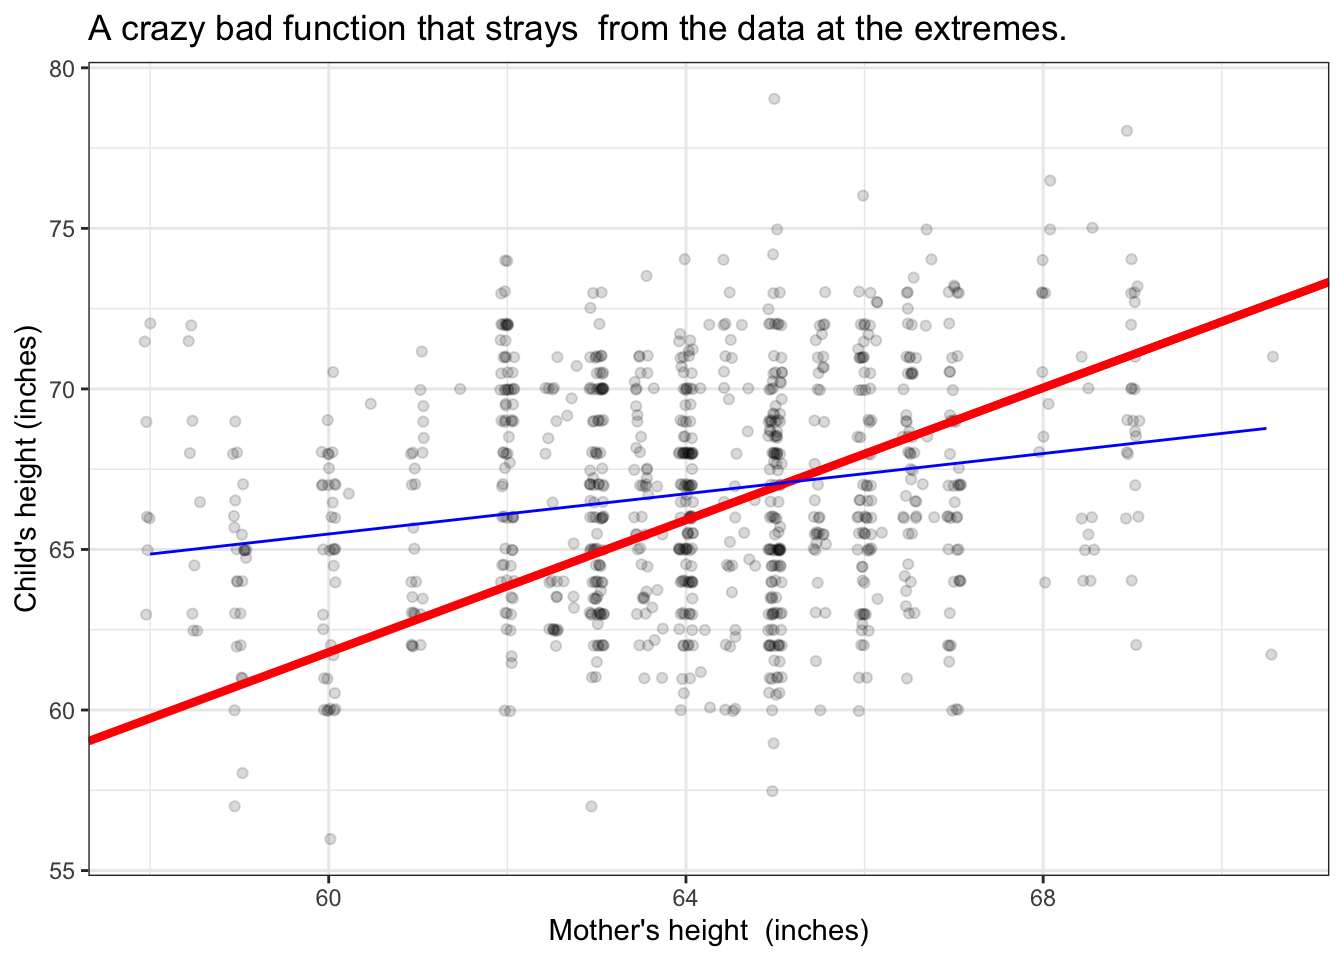
\includegraphics[width=0.8\linewidth]{120-Outside-of-the-normal_files/figure-latex/unnamed-chunk-2-2} 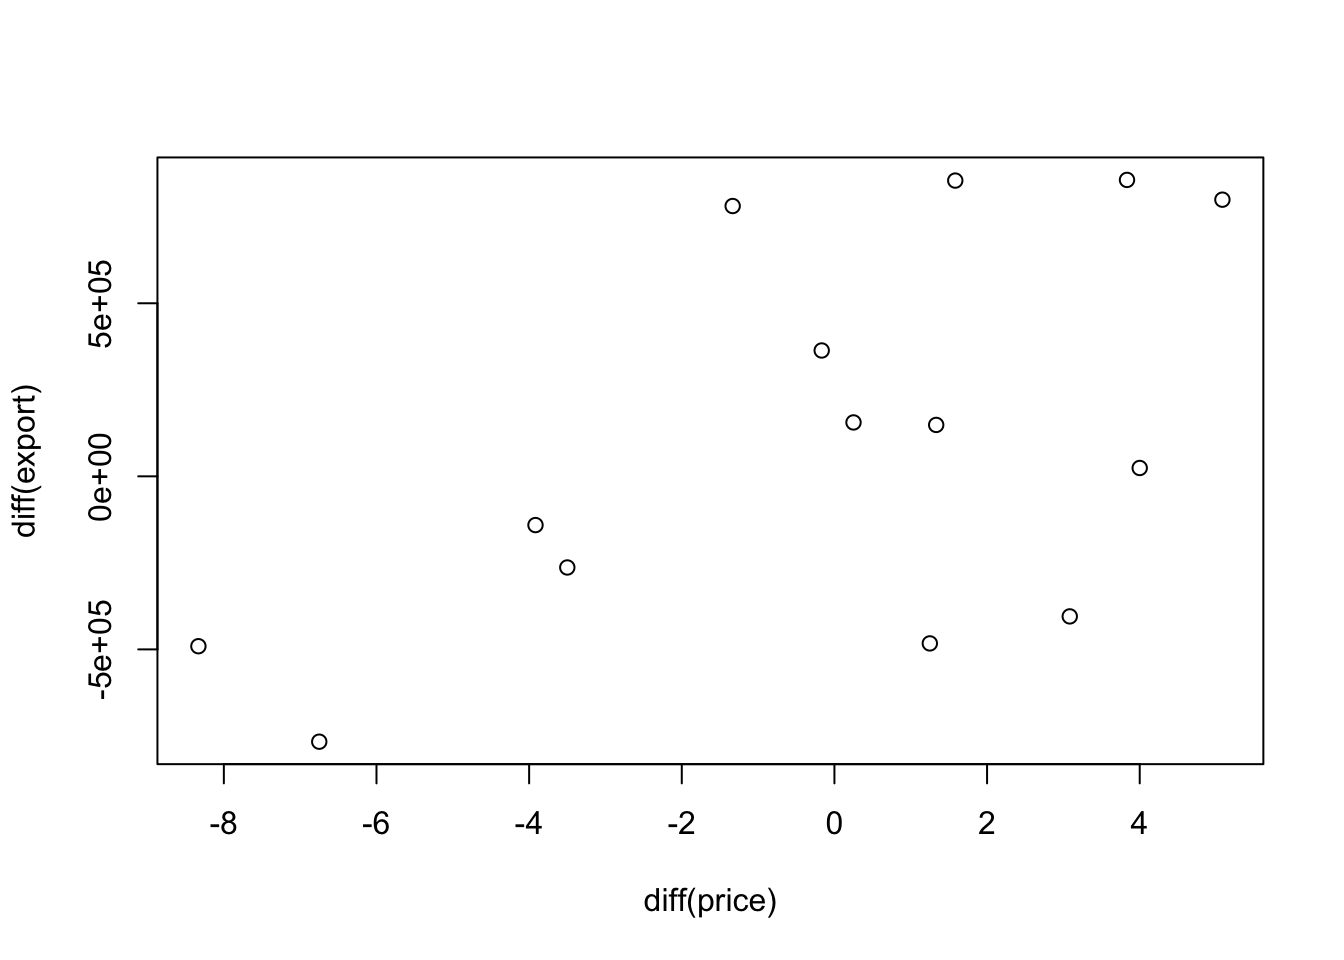
\includegraphics[width=0.8\linewidth]{120-Outside-of-the-normal_files/figure-latex/unnamed-chunk-2-3} 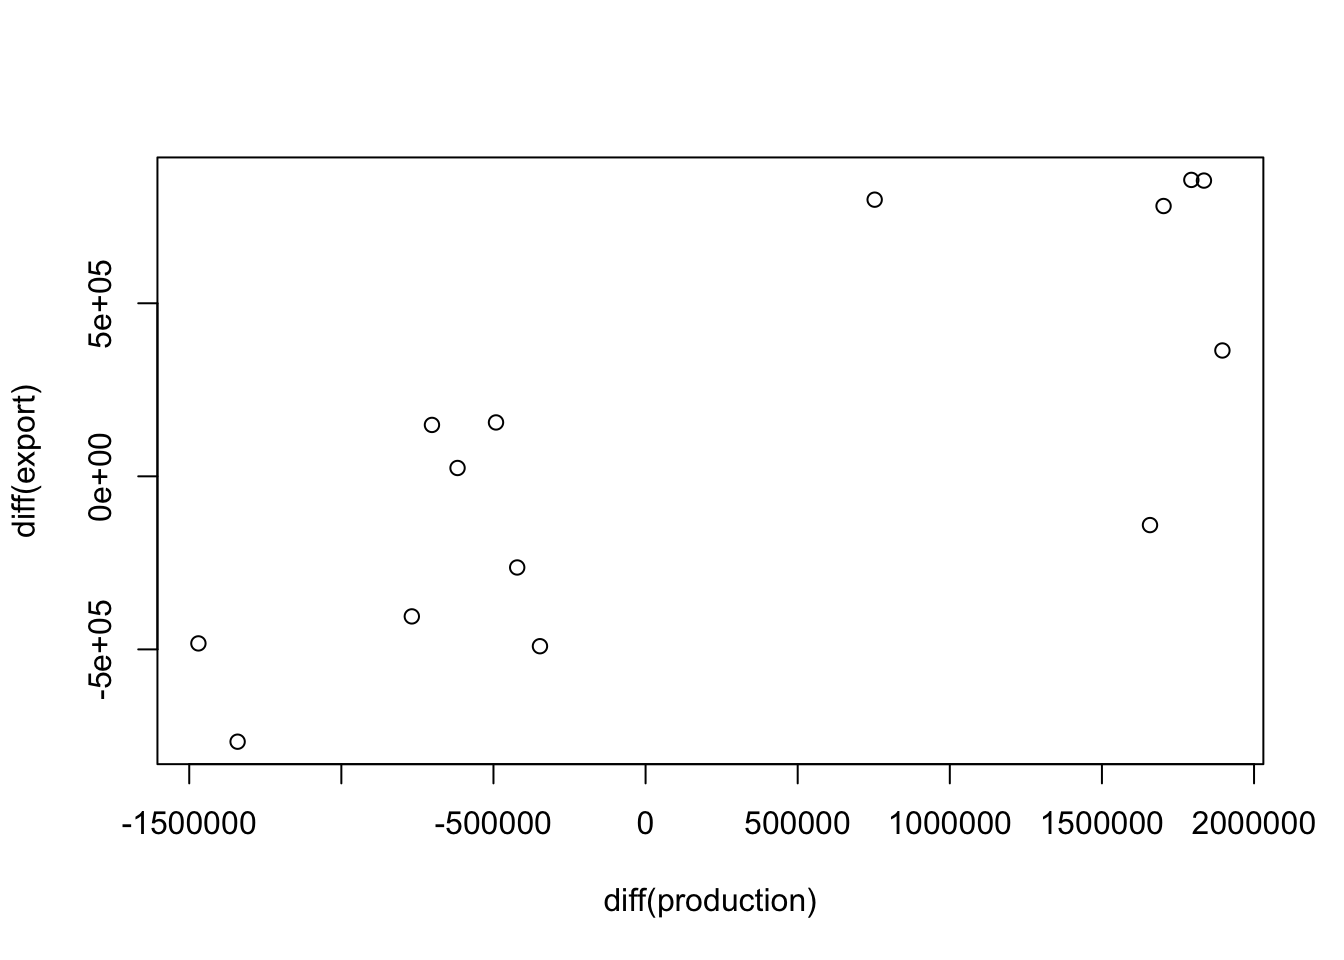
\includegraphics[width=0.8\linewidth]{120-Outside-of-the-normal_files/figure-latex/unnamed-chunk-2-4}

\begin{verbatim}
## 
## Call:
## lm(formula = diff(export) ~ diff(production) + diff(price), data = Wheat_export)
## 
## Residuals:
##     Min      1Q  Median      3Q     Max 
## -438894 -139590   39148  188279  303853 
## 
## Coefficients:
##                   Estimate Std. Error t value Pr(>|t|)    
## (Intercept)      4.301e+04  7.106e+04   0.605 0.557241    
## diff(production) 3.051e-01  5.672e-02   5.379 0.000224 ***
## diff(price)      6.404e+04  1.792e+04   3.574 0.004362 ** 
## ---
## Signif. codes:  0 '***' 0.001 '**' 0.01 '*' 0.05 '.' 0.1 ' ' 1
## 
## Residual standard error: 259500 on 11 degrees of freedom
## Multiple R-squared:  0.8176, Adjusted R-squared:  0.7844 
## F-statistic: 24.65 on 2 and 11 DF,  p-value: 8.629e-05
\end{verbatim}

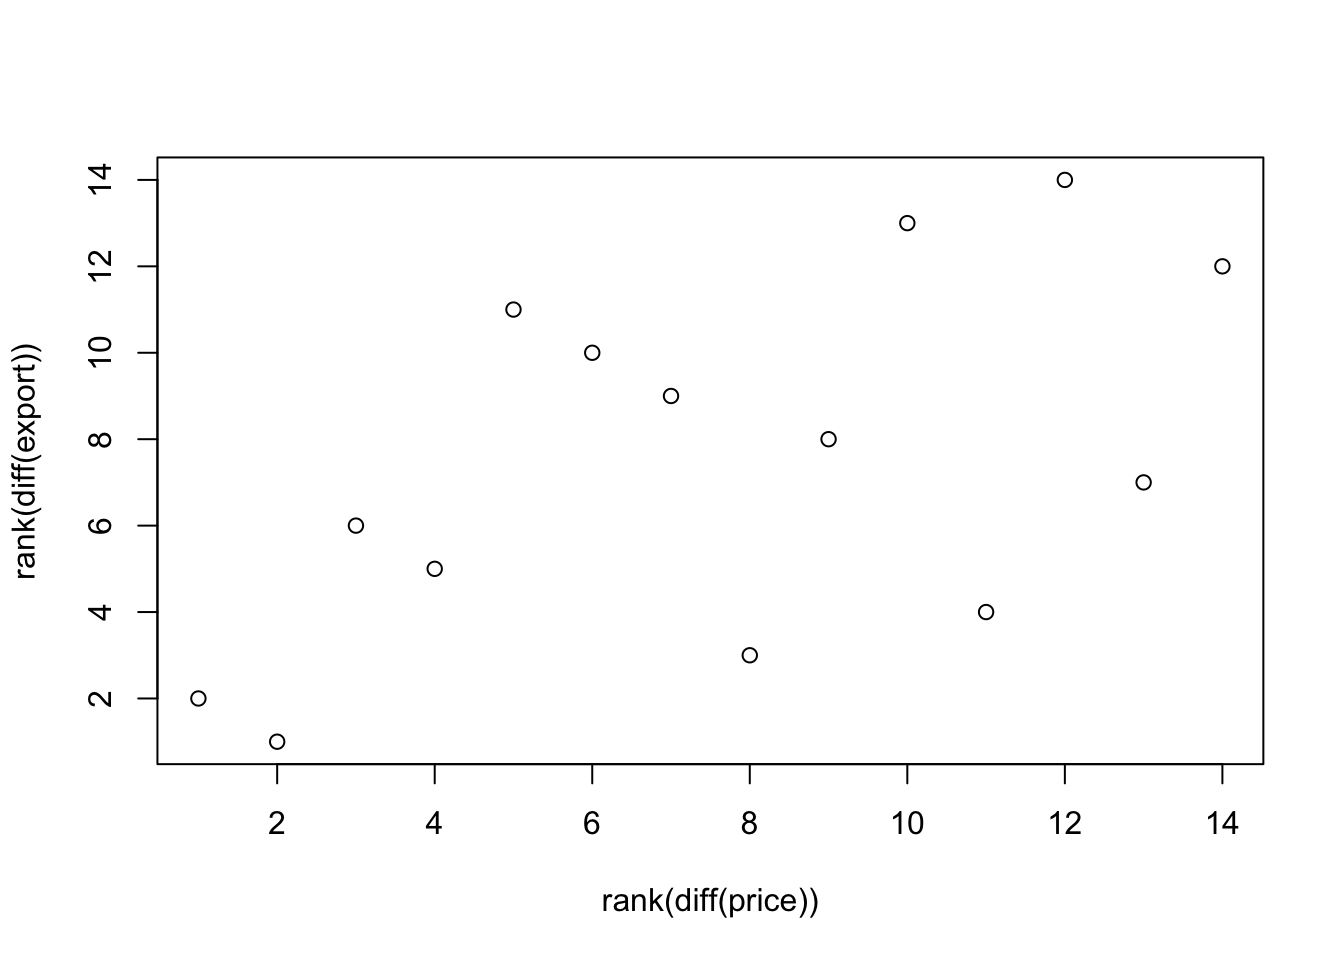
\includegraphics[width=0.8\linewidth]{120-Outside-of-the-normal_files/figure-latex/unnamed-chunk-2-5} 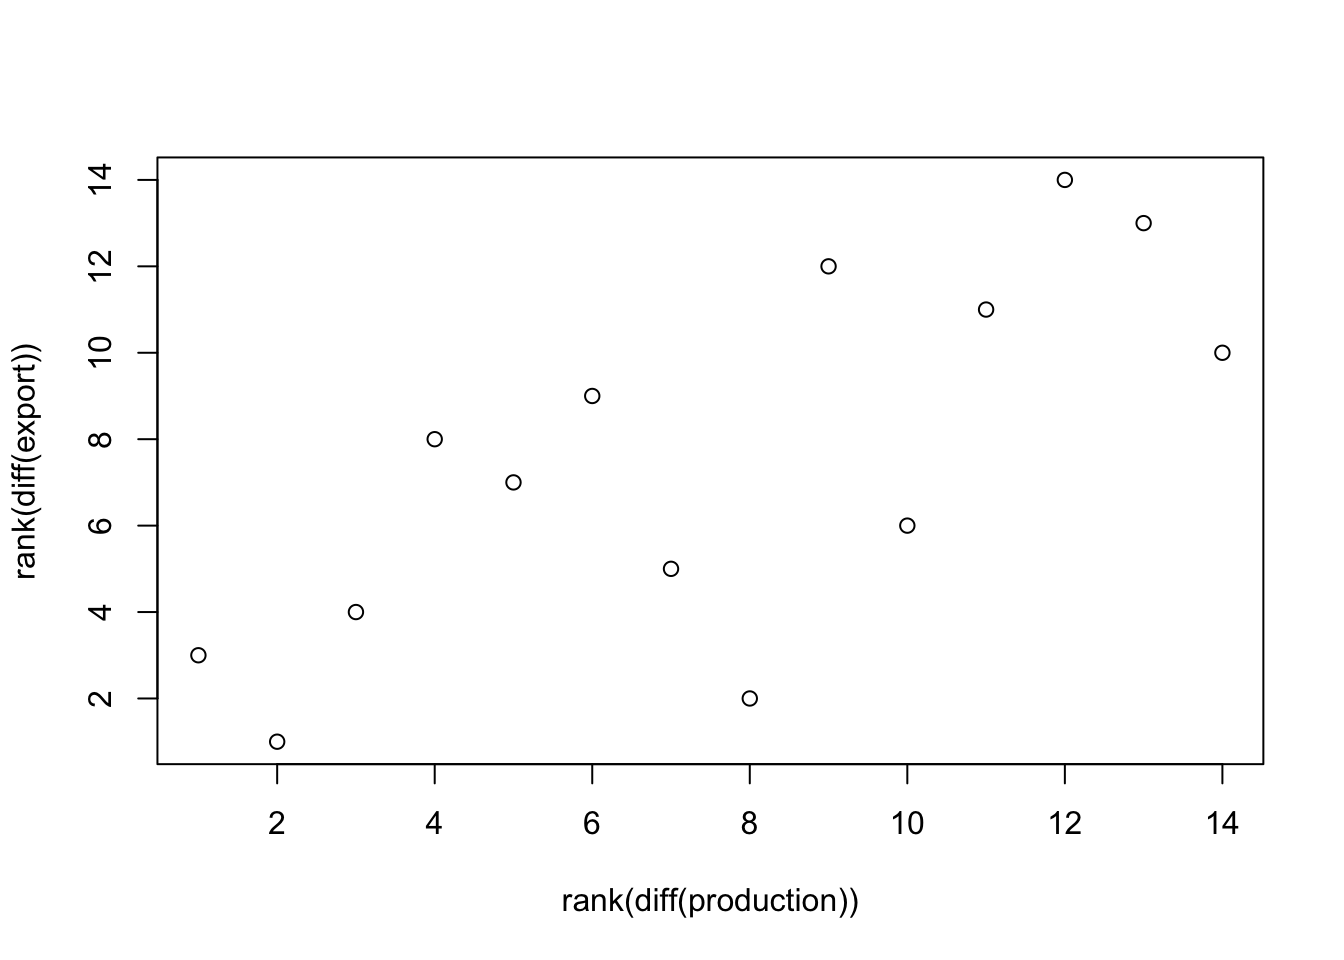
\includegraphics[width=0.8\linewidth]{120-Outside-of-the-normal_files/figure-latex/unnamed-chunk-2-6}

They computed indices, which seem to be the standardized annual differences.

\includegraphics[width=0.8\linewidth]{120-Outside-of-the-normal_files/figure-latex/unnamed-chunk-3-1} 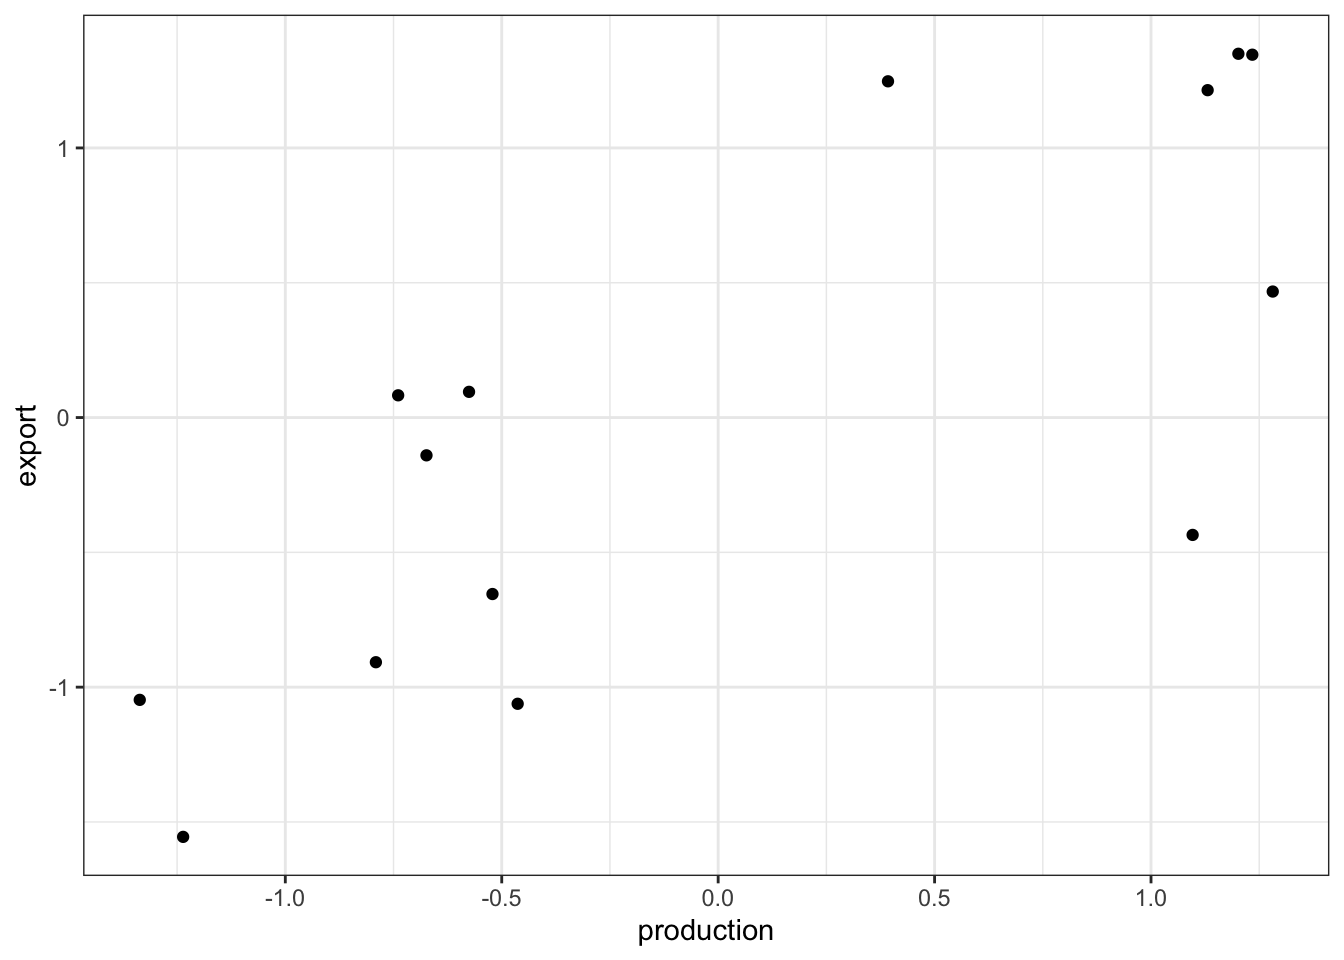
\includegraphics[width=0.8\linewidth]{120-Outside-of-the-normal_files/figure-latex/unnamed-chunk-3-2}

\begin{verbatim}
## 
## Call:
## lm(formula = export ~ price + production, data = Indices)
## 
## Residuals:
##      Min       1Q   Median       3Q      Max 
## -0.78544 -0.24981  0.07006  0.33694  0.54378 
## 
## Coefficients:
##              Estimate Std. Error t value Pr(>|t|)    
## (Intercept) 2.083e-17  1.241e-01   0.000 1.000000    
## price       4.665e-01  1.305e-01   3.574 0.004362 ** 
## production  7.021e-01  1.305e-01   5.379 0.000224 ***
## ---
## Signif. codes:  0 '***' 0.001 '**' 0.01 '*' 0.05 '.' 0.1 ' ' 1
## 
## Residual standard error: 0.4643 on 11 degrees of freedom
## Multiple R-squared:  0.8176, Adjusted R-squared:  0.7844 
## F-statistic: 24.65 on 2 and 11 DF,  p-value: 8.629e-05
\end{verbatim}

What if we do it with log proportional change \ldots{}

\begin{verbatim}
## [1] 0.09435189
\end{verbatim}

\begin{verbatim}
## [1] 0.740655
\end{verbatim}

\includegraphics[width=0.8\linewidth]{120-Outside-of-the-normal_files/figure-latex/unnamed-chunk-4-1} 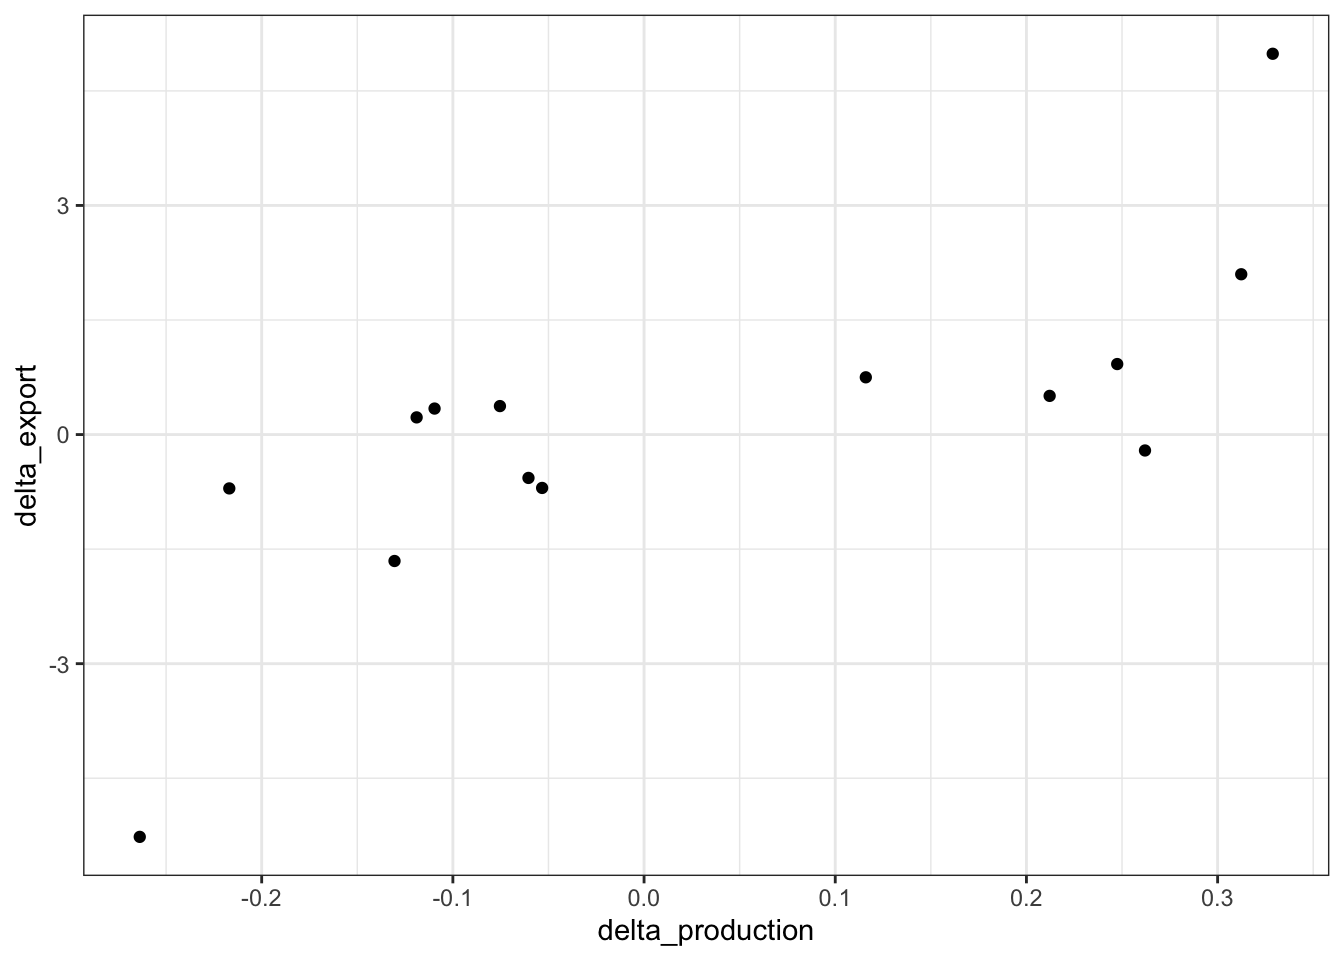
\includegraphics[width=0.8\linewidth]{120-Outside-of-the-normal_files/figure-latex/unnamed-chunk-4-2}

\begin{verbatim}
## 
## Call:
## lm(formula = delta_export ~ delta_price + delta_production, data = Deltas)
## 
## Residuals:
##      Min       1Q   Median       3Q      Max 
## -3.03150 -0.75490 -0.02567  1.22324  2.56527 
## 
## Coefficients:
##                  Estimate Std. Error t value Pr(>|t|)   
## (Intercept)       -0.1720     0.4365  -0.394  0.70114   
## delta_price        0.3642     3.2910   0.111  0.91387   
## delta_production   7.8920     2.1741   3.630  0.00396 **
## ---
## Signif. codes:  0 '***' 0.001 '**' 0.01 '*' 0.05 '.' 0.1 ' ' 1
## 
## Residual standard error: 1.607 on 11 degrees of freedom
## Multiple R-squared:  0.5491, Adjusted R-squared:  0.4671 
## F-statistic: 6.697 on 2 and 11 DF,  p-value: 0.01252
\end{verbatim}

\hypertarget{remember-inference-isnt-everything}{%
\chapter{Remember, inference isn't everything}\label{remember-inference-isnt-everything}}

Study design, sampling bias, etc.

\hypertarget{refs}{}
\leavevmode\hypertarget{ref-punnett-1905}{}%
Bateson, W., E.R. Saunders, and R.C. Punnett. 1905. ``Experimental Studies in the Physiology of Heredity.'' \emph{Reports to the Evolution Committee of the Royal Society} 2: 1--55, 80--99.

\leavevmode\hypertarget{ref-ISRS}{}%
Diez, David, Christopher Barr, and Mine Çetinkaya-Rundel. 2014. \emph{Introductory Statistics with Randomization and Simulation}. OpenIntro.org. \url{https://www.openintro.org/download.php?file=isrs1_tablet\&referrer=/stat/textbook.php}.

\leavevmode\hypertarget{ref-modern-dive}{}%
Ismay, Chester, and Albert Y. Kim. 2019. \emph{Statistical Inference via Data Science: A Moderndive into R and the Tidyverse}. CRC Press. \url{https://moderndive.com}.

\leavevmode\hypertarget{ref-lock5}{}%
Lock, Robin H., Patti Frazer Lock, Kari Lock Morgan, Eric F. Lock, and Dennis F. Lock. 2017. \emph{Statistics: Unlocking the Power of Data}. 2nd ed. Wiley.

\leavevmode\hypertarget{ref-tintle-investigations}{}%
Tintle, Nathan, Beth L. Chance, Soma Roy, George W. Cobb, Allan J. Rossman, Todd Swanson, and Jill VanderStoep. 2016. \emph{Introduction to Statistical Investigations}. Wiley.



\end{document}
